% !Mode:: "TeX:UTF-8"
% !TEX program  = xelatex

\documentclass[withoutpreface,bwprint]{cumcmthesis}
%\documentclass[withoutpreface,bwprint]{cumcmthesis} %去掉封面与编号页,电子版提交的时候使用。


\usepackage[framemethod=TikZ]{mdframed}
\usepackage{url}   % 网页链接
\usepackage{subcaption} % 子标题
\title{基于灰色模糊网络分析法的信贷决策模型} % 大标题
\tihao{} % 题号
\baominghao{}
\schoolname{}
\membera{}
\memberb{}
\memberc{}
\supervisor{}
\yearinput{}
\monthinput{}
\dayinput{}

\begin{document}

\maketitle
\begin{abstract}
    ``中小微企业信贷难''一直是近年来困扰中小微企业和各大银行的问题。
    由于中小微企业自身存在``规模较小''、``缺乏抵押资产''等弱点,
    银行难以对其信贷风险进行全面、完整的评估。本文就中小微企业的信贷风险评估、
    银行的信贷策略和银行的信贷应急调整策略等问题进行分析与讨论。\par
    \textbf{针对问题一}\quad 
        我们首先确定出九个信贷风险评价指标,并运用 $F - ANP$ 方法确定各指标权重。然后我们运用灰色
        综合评价方法,将各风险指标评分进行白化,以此求出灰色评价系数和灰色评价矩阵。将已求得的各指标权重向量、灰色评价矩阵和风险划分标准向量相乘得到企业
        信贷风险评估值,以此作为企业信贷风险量化分析值。然后,我们将企业信贷风险评估值散列在 $\left[1 - 10\right]$ 整数区间内,来确定企业信贷风险等级,并
        由企业年收入、年利润和信贷风险等级综合确定企业贷款额度百分比。最后,我们拟合出附件 3 中 ``客户流失率'' 与 ``贷款年利率'' 之间的函数关系,以银行未来三年
        的贷款利率收益和为目标函数,求出目标函数最大时对应的贷款年利率值,以此作为基准贷款年利率。再根据企业信贷风险评估值对企业实际贷款年利率进行不同程度上浮调整,
        最终得出各企业贷款年利率。企业贷款额度百分比和企业贷款年利率共同构成银行对这 123 家企业的信贷策略。(具体答案数据见附录 A 、附录 B )\par
    \textbf{针对问题二}\quad
        我们以第一问建立的基于灰色模糊网络分析法的信贷决策模型为基础,将附件 2 中所给出的 302 家企业的数据代入模型,计算出各企业的信贷风险值、信贷风险等级和贷款额度百分比。
        我们将贷款额度收束到题目要求的区间,并进行归一化处理得到最终的贷款额度百分比。
        然后,我们基于自己的理解和对问题二的适应性对国际银行业主流的 $RAROC$ 贷款定价模型进行改进,然后运用改进后的 $RAROC$ 对银行基准贷款年利率评估做进一步优化。
        再通过综合考虑银行收入、成本和预期损失等因素,以 $RAROC$ 函数为目标函数、以不良贷款率不超过一定值为约束条件,进行规划,求得银行信贷基准利率,
        再根据企业信贷风险评估值对企业实际贷款年利率进行不同程度上浮调整,最终得出 302 家企业的实际信贷利率,结合企业信贷额度即为银行对这 302 家企业的信贷策略。(具体答案数据见附录 C 、附录 D )\par
    \textbf{针对问题三}\quad
        我们以新冠疫情这一突发因素为例,先定性分析新冠疫情下我国各行业的发展现状和未来发展前景,以这两项指标去修正问题一中确定企业贷款额度百分比的模型,
        从而确定新冠疫情突发情况下各企业贷款额度百分比。我们再沿用 $RAROC$ 模型去确定银行信贷基准利率,
        综合考量企业未来和国家政策扶持等影响因素,最终确定企业的贷款额度和实际信贷利率。我们还简要分析了在科研领域取得突破、科研产品迅速投入市场的突发情况下,
        银行对 302 家企业信贷策略的变化。
        (具体答案数据见附录 E )\par
    \textbf{关键词 \quad 灰色系统 \quad $ANP$ 网络分析法 \quad 三角模糊 \quad $RAROC$ 贷款定价模型 \quad} % 关键词三到五个为宜
    \end{abstract}

    \section{问题重述}
    \subsection{问题背景}\par
    个体工商户和中小微企业是零售银行战略中非常重要的客户群。但由于中小微企业自身规模较小且缺乏抵押资产,所以银行通常是根据信贷政策、企业的交易票据信息和上下游企业的影响力 \cite{魏晓彬2014} ,向\textbf{实力强}、\textbf{供求关系稳定}的企业提供贷款,并可以对\textbf{信誉高}、\textbf{信贷风险小}的企业给予利率优惠。银行首先根据中小微企业的实力、信誉对其信贷风险做出评估\cite{柏群,曹华玲2012},然后依据信贷风险等因素来确定\textbf{是否放贷及贷款额度、利率和期限}等信贷策略。
    
    \subsection{问题的提出}\par
    某银行对确定要放贷企业的贷款额度为 10 -- 100万元,年利率控制在 4\% -- 15\% ,贷款期限为 1 年。根据附件 1 -- 3 中有信贷记录企业、无信贷记录企业的信誉评级、进项发票信息和销项发票信息等相关信息,通过建立信贷风险评估数学模型,解决以下三个问题:
    \begin{problem}
        对附件 1 中 123 家企业的信贷风险进行量化分析,给出该银行在年度信贷总额固定时对这些企业的信贷策略。
    \end{problem}
    \begin{problem}
        在问题 1 的基础上,对附件 2 中 302 家企业的信贷风险进行量化分析,并给出该银行在年度信贷总额为 1 亿元时对这些企业的信贷策略。
    \end{problem}
    \begin{problem}
        综合考虑附件 2 中各企业的信贷风险和可能的突发因素(例如:新冠病毒疫情)对各企业的影响,给出该银行在年度信贷总额为 1 亿元时的信贷调整策略。
    \end{problem}
    附件1 123 家有信贷记录企业的相关数据 \\
    附件2 302 家无信贷记录企业的相关数据 \\
	附件3 银行贷款年利率客户流失率关系的 2019 年统计数据

    \subsection{数据预处理}\par
    \begin{enumerate}
        \item 作废发票是指因故取消交易而使发票作废,其对企业信誉评估几乎不产生影响,所以对附件1、附件2中作废发票数据项予以剔除。
        \item 附件1、2中开票日期均以日为单位且不连续,不便于后续分析。所以我们对不同数据项进行按月累加、求标准差等操作,得到以月份为单位的相关数据。
    \end{enumerate}

    \section{问题分析}
    \subsection{问题一的分析}
        问题一要求根据附件 1 中给出的企业信誉评级和进项发票信息、销项发票信息,对企业信贷风险进行量化分析并制定相应的银行信贷策略。\par
        我们采用基于三角模糊数的灰色网络分析法来确定各企业风险评估分数,并根据企业年收入、年利润和信贷风险等级来确定企业的信贷额度百分比。我们依据潜在客户流失率等指标给出该银行对企业的信贷基准利率,再根据企业风险评估分数
        来调整得出各企业实际贷款利率,从而确定最终的银行信贷策略。\par
        具体而言,我们根据题目要求确定信贷风险指标集$Z$和风险评语集$K$,然后构造基于三角模糊数的模糊判断矩阵$P$并据此确定加权超矩阵$W$,将加权超矩阵$W$进行
        无穷次\footnote{理论上需要计算无穷次幂,实际计算时设置可容忍误差精度,当迭代至实际误差精度小于可容忍误差精度时,即可停止计算并得出结果。}迭代得到二级指标权重$\omega$。
        然后,我们构建风险指标评分样本矩阵,并依据线性白化权函数$f$将风险指标白化,求出灰色评价系数和灰色评价矩阵。最后将已求得的二级指标权重向量$\omega$、灰色评价矩阵$X$和风险划分标准向量$K$相乘,
        得到风险值$F$,汇总得出 123 家企业的信贷风险量化分析表。(见附录 A )\par
        我们根据已求得的企业风险评估值$F$,来确定企业信贷风险等级(见附录 A ),由企业年收入、年利润和信贷风险等级综合确定企业贷款额度百分比。\par
        我们根据附件 3 中数据,分别建立不同信誉评级的``客户流失率''与``贷款年利率''之间的函数关系。
        以银行连续贷款三年为例,计算不同利率下的银行总收益,并以最大总收益对应的贷款年利率为银行基准贷款年利率。
        然后根据以求得的企业风险评估值$F$,建立奖惩机制,对不同风险评级的企业予以一定程度上贷款利率的浮动,最终得出各企业的贷款利率\cite{姜启源,谢金星,叶俊2017}。
    \subsection{问题二的分析}
        问题二要求以问题一模型为基础,对附件 2 中 302 家企业的信贷风险进行量化分析,并给出该银行在年度信贷总额为 1 亿元时对这些企业的信贷策略。
        我们以问题一中建立的数学模型为基础,将附件 2 中企业数据代入,解得相应的信贷风险值、信贷风险等级和贷款额度百分比。我们对问题一模型中求解各企业
        信贷利率的方法进行优化,采用国际银行业主流的 $RAROC$ 贷款定价模型进行计算,得出银行信贷基准利率,最后再次利用问题一中相同的方法求出各企业实际信贷利率。
        综合企业信贷额度和实际信贷利率,即为银行信贷策略。
    \subsection{问题三的分析}
        问题三要求分析可能的突发因素对各企业的影响,并给出该银行在年度信贷总额为 1 亿元时的信贷调整策略。\par
        以新冠疫情为例,我们系统分析了新冠疫情下各行各业的现状和未来发展能力,再在第二问模型的基础上添加发展前景指标,从而以企业年收入、年利润、信誉评级和发展前景四个指标
        来衡量贷款额度。我们沿用 $RAROC$ 模型去确定银行基准贷款利率,再根据企业信誉评级进行利率奖惩,又因为国家扶持中小微企业贷款政策的影响,对各个行业的整体利率均按照不同程度进行下调,
        最终给出 附件 2 中 302 家企业的贷款额度和实际贷款利率。(见附录 E )        
    
    \section{模型流程图}
    \begin{figure}[H]
        \begin{center}
            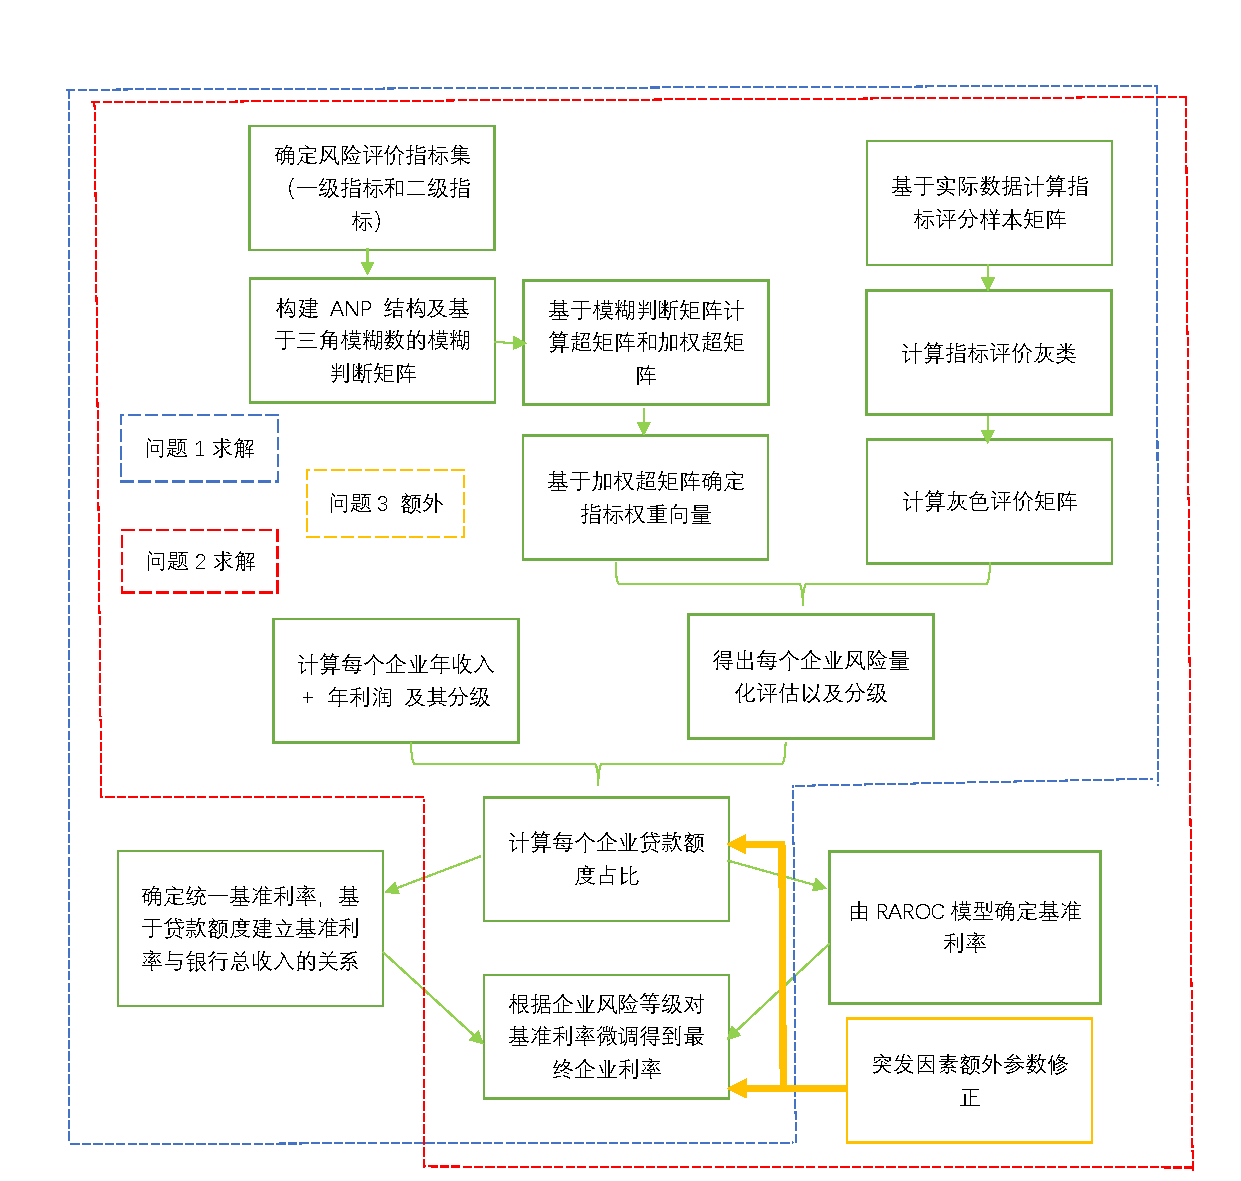
\includegraphics[width = 1.0\textwidth, height = 0.5\textheight]{流程图.pdf}
            \caption{流程图}
        \end{center}
    \end{figure} 

    \section{模型假设}
    \begin{enumerate}
        \item 默认社会的整体经济状况稳定,短期内没有政策改变或突发情况使得企业的销项和进项发生改变,企业销项和进项的变化均只受市场自由调节。
        \item 因为中小微企业发展规模较小,默认中小微企业没有科研投入,即同一产品成本无法降低,企业进项的额度减少只能因为购买产品的数目减少。
        \item 默认企业遵纪守法,所有销售和购买行为均开具发票且记录在册,企业无其他额外收入。
        \item 中小企业规模较小,且缺少抵押资产,企业无在其他银行贷款行为,所以该银行采取同一种贷款产品。对于同一种贷款产品,银行为了维护金融行业的稳定性,所以不同公司、不同贷款额度的贷款利率差距不能过大,本模型假设利率在基准利率上下浮动范围为 0.5 -- 2 个百分点。
        \item 默认将市场上信誉最好企业的贷款利率定为基准利率,并在此基础上上浮 0.5 -- 2 个百分点作为浮动利率的范围。
    \end{enumerate}
    
    \section{符号说明}
    \begin{center}
        \begin{tabular}{>{\centering}p{6em}>{\centering\arraybackslash}p{30em}}
            \toprule
            符号 & 说明 \\
            \midrule
            $f_i$ & 第$i$类白化权函数 \\
            $p_{ij}$ & 以对第三指标的影响为标准,指标$i$比指标$j$的相对重要程度 \\
            $\omega_{ij}$ & 加权超矩阵$W$中元素,表示元素$i$对元素$j$的影响程度\\
            $Z_{i}$ & 第$i$个一级风险评价指标 \\
            $Z_{ij}$ &  第$i$个一级风险评价指标中的第$j$个二级风险评价指标\\
            $K_i$ & 第$i$项风险评级 \\
            $M$ & 元素组的相对权重矩阵 \\
            $T_i$ & 第$i$灰类总评价系数 \\
            $F_i$ & 第$i$家企业信贷额度值 \\
            $S_i$ & 第$i$类信誉评级的``客户流失率''随``贷款年利率''的变化函数 \\
            \bottomrule
        \end{tabular}
    \end{center} 
    注:其他符号含义将在论文中第一次出现时进行解释。
    
    \section{问题一建模与求解}
    \subsection{灰色综合评价法理论基础}
        灰色综合评价法\cite{张波2013}建立在灰色系统理论的基础上,可对``部分信息明确,部分信息未知''的小样本
        进行研究,通过对已有信息的分析,提取出有用信息,实现最终的决策。 \par
        灰色模型的建模思想是利用序列算子或灰色生成的作用弱化数据的随机性,发现潜在规律,经灰色微分方程
        和差分方程间的互换,将离散数据序列构造成连续的动态微分方程。\par
        本文应用的灰色评价方法是灰色统计法和灰色关联分析法。灰色统计法通过引入白化函数将一些具体数据按所属灰类
        进行整理归纳,得出统计指标所属灰类,通俗的讲就是根据评估点的情况对评估指标进行分析,最终得出评估指标的
        聚类。灰色关联分析法是根据系统各因素集间发展趋势曲线相似或相异程度来表现系统各因素集间的关联度。发展趋势曲线
        集合形状越相似,则关联度越大,反之越小。
    \subsection{三角模糊数}
        风险评价过程中,学术界对确定各指标权重时多采用固定比值表示两元素间的重要性,
        这种方式体现了对比两元素间重要程度的\textbf{绝对性}。然而在实际生活中,指标间的重要程度量化值往往并不是绝对的,
        其存在\textbf{最悲观值}、\textbf{最可能值}、\textbf{最乐观值},这三个值的同时存在能够使得到的评价结果更加客观。
        因此,在确定指标重要性程度时,我们引入``三角模糊数''理论\cite{ZENG2007137}。
        \subsubsection{三角模糊数定义}
            设某模糊变量$p$的\textbf{下限}、\textbf{最可能值}和\textbf{上限} 分别为三个实数$a$、$b$、$c$,且存在$0 \leq a \leq b \leq c \leq 1$,则这个三角模糊数表示为
            $ p = (a, b, c)$。
        \subsubsection{三角模糊数性质}
            设两个三角模糊数为$p_1 = (a_1, b_1, c_1), p_2 = (a_2, b_2, c_2)$,则有相关运算法则:
            \begin{gather}
                p_{1}+p_{2}=\left(a_{1}, b_{1}, c_{1}\right)+\left(a_{2}, b_{2}, c_{2}\right)=\left(a_{1}+a_{2}, b_{1}+b_{2}, c_{1}+c_{2}\right) \\
                p_{1} \times p_{2}=\left(a_{1}, b_{1}, c_{1}\right) \times\left(a_{2}, b_{2}, c_{2}\right)=\left(a_{1} \times a_{2}, b_{1} \times b_{2}, c_{1} \times c_{2}\right) \\
                \frac{1}{p_{1}}=\left(\frac{1}{a_{1}}, \frac{1}{b_{1}}, \frac{1}{c_{1}}\right) \\
                \lambda p_{1}=\left(\lambda a_{1}, \lambda b_{1}, \lambda c_{1}\right) \quad \text { 其中 } \lambda>0
            \end{gather}
        \subsubsection{三角模糊数构建互补判断矩阵}
            设判断矩阵$p = (p_{ij})_{n \times n}$,其中$p_{ij} = (a_{ij}, b_{ij}, c_{ij})$,$p_{ji} = (a_{ji}, b_{ji}, c_{ji})$。\par
            若同时满足$a_{ii} = b_{ii} = c_{ii} = 0.5$ 和 $a_{ij} + c_{ji} = b_{ij} + b_{ji} = c_{ij} + a_{ji} = 1$,则我们称$p$为三角
            模糊数互补判断矩阵,其中$p_{ij}$表示以对第三指标的影响为标准,指标$i$比指标$j$的相对重要程度。\par
            进行风险评价时,$p_{ij}$中的$(a_{ij}, b_{ij}, c_{ij})$分别表示指标$i$比指标$j$的相对重要程度的最悲观值、最可能值和最乐观值。
            其中$a_{ij}$、$c_{ij}$决定着整体的模糊程度,两者相差越大,则判断越模糊。反之,模糊程度越小。当两者相等时,则表示为明确信息,不存在模糊度。\par
            三角模糊数的取值我们采用0.1 -- 0.9的标度方法,其代表具体含义见表\ref{表:三角模糊数取值表及含义解释}:
            \begin{table}[H] \begin{center}
                \begin{tabular}{>{\centering}p{6em}>{\centering\arraybackslash}p{30em}}
                    \toprule
                    标度 & 解释 \\
                    \midrule
                    0.1 & 两因素比较,前者相对后者\emph{极端不}重要 \\
                    0.2 & 两因素比较,前者相对后者\emph{很不}重要 \\
                    0.3 & 两因素比较,前者相对后者\emph{一般不}重要 \\
                    0.4 & 两因素比较,前者相对后者\emph{略微不}重要 \\
                    0.5 & 两因素比较,前者相对后者\emph{同等}重要 \\
                    0.6 & 两因素比较,前者相对后者\emph{略微}重要 \\
                    0.7 & 两因素比较,前者相对后者\emph{一般}重要 \\
                    0.8 & 两因素比较,前者相对后者\emph{很}重要 \\
                    0.9 & 两因素比较,前者相对后者\emph{极端}重要 \\
                    \bottomrule
                \end{tabular}
                \caption{三角模糊数取值表及含义解释}
                \label {表:三角模糊数取值表及含义解释}
            \end{center} \end{table}


    \subsection{基于三角模糊数的灰色网络分析法}
        \subsubsection{风险评价指标集合风险评语集}
            \begin{enumerate}
                \item 确定风险评价指标集 \par
                      企业信贷风险有$n_1(n_1 = 3)$个一级指标。一级风险评价因素集为:
                      \begin{align*}
                        Z = \{Z_1, Z_2, Z_3\} = \{\text{公司状况},\text{盈利偿债能力},\text{运营发展能力}\}
                      \end{align*}
                      二级风险评价因素集为:
                      \begin{align*}
                        Z_1 &= \{Z_{11}, Z_{12}\} \phantom{, Z_{13}, Z_{14}} = \{\text{公司类型}, \text{信誉情况}\} \\
                        Z_2 &= \{Z_{21}, Z_{22}, Z_{23} \} \phantom{, Z_{24}} = \{\text{总净利率}, \text{成长性\footnote{成长率指收入增长率与支出增长率的比值}}, \text{月平均盈利}\} \\
                        Z_3 &= \{Z_{31}, Z_{32}, Z_{33}, Z_{34} \} = \{\text{利润标准差}, \text{收入增长率}, \text{供关系\footnote{供关系指下游企业对该企业的用户粘度}}, \text{求关系\footnote{求关系指该企业对上游企业的用户粘度}}\} 
                      \end{align*}
                \item 确定风险评语集\par 
                      风险评语是对各评级指标所处风险等级的一种语言描述,是资深专家或官方给出的对指标风险等级的判断。
                      为了计算方便,需要将其进行量化,本文将风险等级分为五个级别,各风险级别对应五个分值,具体如下:
                      \[K = \{\text{优秀,良好,一般,合格,不合格}\} = \{1, 2, 3, 4, 5\}\]
            \end{enumerate}
        \subsubsection{建立网络层次结构}
            综合考虑各风险评价指标之间的相互作用关系,建立信贷企业的风险评价网络层次结构如图 \ref{图:风险评价网络层次图} 所示:
            \begin{figure}[H]
                \begin{center}
                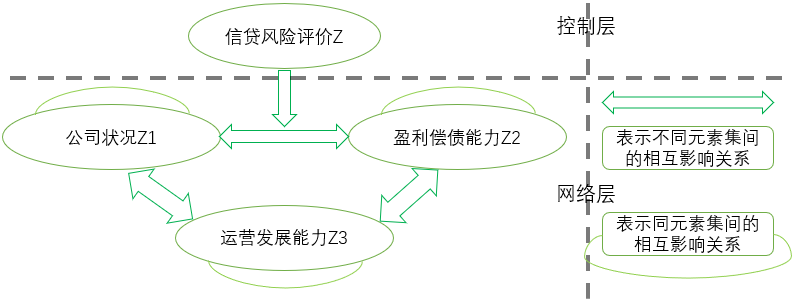
\includegraphics[width = 1.0\textwidth]{风险评价网络层次图.png}
                \caption{风险评价网络层次图}
                \label {图:风险评价网络层次图}
                \end{center}
            \end{figure}
        \subsubsection{$F - ANP$确定指标权重}
            \begin{enumerate}
                \item 构建$ANP$结构 \par
                      根据上文中确定的风险评价指标集,建立风险评价的网络层次结构。在网络结构中,控制层需要确定一个评价目标和准则层的个数,
                      网络层还需要确定各指标集间的相互作用关系。其可分为相互独立的关系,即两指标集之间不存在相互影响;非独立关系,即
                      指标之间相互影响。
                \item 构造基于三角模糊数的模糊判断矩阵 \par
                      以元素组$Z_2$为例,在某一准则情况下,以对$Z_2$中的元素$Z_{22}(i = 1, 2, 3, \dots, n_1)$的影响程度为次准则,根据标度表和三角模糊数的基本理论构造两两互补判断矩阵$P_{22}$为:\par
                        \begin{equation}
                        P_{22}=\left[p_{i j}\right]_{n_{1} \times n_{2}}=\left[
                            \begin{array}{ccccc}
                                p_{11} & p_{12} & p_{13} & \cdots & p_{1 n_{2}} \\
                                p_{21} & p_{22} & p_{23} & \cdots & p_{2 n_{2}} \\
                                p_{31} & p_{32} & p_{33} & \cdots & p_{3 n_{2}} \\
                                \vdots & \vdots & \vdots & \ddots & \vdots \\
                                p_{n_{1} 1} & p_{n_{1} 2} & p_{n_{1} 3} & \cdots & p_{n_{1} n_{2}}
                            \end{array}\right]
                        \end{equation}
                        其中$P_{ij} = (a_{ij}, b_{ij}, c_{ij})$是根据国内外专家对相关指标相对重要程度的评判,经过模糊处理转化得来。
                        代入数据得:
                        \begin{equation*}
                        P_{22}=\left[
                            \begin{array}{ccc}
                                (0.5,0.5,0.5) & (0.2,0.3,0.4) & (0.8,0.8,0.9) \\
                                (0.6,0.7,0.8) & (0.5,0.5,0.5) & (0.4,0.6,0.6) \\
                                (0.1,0.2,0.2) & (0.4,0.4,0.6) & (0.5,0.5,0.5)
                            \end{array}\right]
                        \end{equation*}
                \item 确定加权超矩阵
                      设$W_{22}$表示在某一准则下,以元素组$Z_2$中某一元素$Z_{2i}(i = 1, 2, 3, \dots, n_2)$的影响程度为次准则,通过计算得出的$Z_2$中元素重要程度。具体计算过程如下:\par
                      第一步:计算$Z_{2i}(i = 1, 2, 3, \dots, n_2)$的综合重要程度$V_{2i}$:
                      \begin{equation}
                        V_{2i} = \sum_{j=1}^{n_2} p_{i j} \otimes\left[\sum_{i=1}^{n_1} \sum_{j=1}^{n_2} p_{i j}\right]^{-1}\left(i=1,2, \cdots, n_{1} ; j=1,2, \cdots, n_{2}\right)
                        \label {公式:综合重要程度V}
                      \end{equation}
                      \phantom{第一步:}公式(\ref{公式:综合重要程度V})中:
                      \begin{equation*}
                        \sum_{j=1}^{n_{2}} p_{i j}=\left(\sum_{j=1}^{n_{2}} a_{i j}, \sum_{j=1}^{n_{2}} b_{i j}, \sum_{j=1}^{n_{2}} c_{i j}\right)
                      \end{equation*}
                      \begin{align*}
                        \left[\sum_{i=1}^{n_{1}} \sum_{j=1}^{n_2} p_{i j}\right]^{-1} &= \left[\sum_{i=1}^{n_{1}} \sum_{j=1}^{n_{2}} a_{i j} \sum_{i=1}^{n_{1}} \sum_{j=1}^{n_{2}} b_{i j} \sum_{i=1}^{n_{1}} \sum_{j=1}^{n_{2}} c_{i j}\right]^{-1}\\
                        &= \left(\frac{1}{\sum_{i=1}^{n_{1}} \sum_{j=1}^{n_{2}} c_{i j}}, \frac{1}{\sum_{i=1}^{n_{1}} \sum_{j=1}^{n_{2}} b_{i j}}, \frac{1}{\sum_{i=1}^{n_{1}} \sum_{j=1}^{n_{2}} \alpha_{i j}}\right)
                      \end{align*}
                      \phantom{第一步:}代入数据得:
                      \begin{align*}
                          V_{21} = (0.300, 0.355, 0.450)\\
                          V_{22} = (0.300, 0.450, 0.525)\\
                          V_{23} = (0.200, 0.244, 0.325)
                      \end{align*}
                      第二步:求$V_{2i} \geq V_{2f}$的可能性程度$R(V_{2i} \geq V_{2f})$:
                      \begin{equation}
                        R(V_{2i} \geq V_{2f})=
                        \left\{
                            \begin{array}{cc}
                            1 & b_{ij}^{2i} \geq b_{ij}^{2f} \\
                            \frac{c_{ij}^{2i} - a_{ij}^{2f}}{c_{ij}^{2i} - a_{ij}^{2f} + b_{ij}^{2f} - b_{ij}^{2i}} & b_{ij}^{2f} \geq b_{ij}^{2i}, a_{ij}^{2f} \leq c_{ij}^{2i} \\
                            0 & \text{其他}
                            \end{array}\right.
                        \label {公式:可能性程度R}
                      \end{equation}
                      \phantom{第二步:}公式(\ref{公式:可能性程度R})中$i\text{、}f = 1, 2, \dots, n_2$ 且 $i \neq f$。 \par
                      \phantom{第二步:}代入数据得:
                      \begin{align*}
                          R(V_{21} \geq V_{22}) &= \frac{0.450 - 0.300}{0.450 - 0.300 + 0.450 - 0.355} = 0.612 & R(V_{21} \geq V_{23}) &= 1\\
                          R(V_{22} \geq V_{21}) &= 1 & R(V_{22} \geq V_{23}) &= 1\\ 
                          R(V_{23} \geq V_{21}) &= \frac{0.325 - 0.300}{0.325 - 0.300 + 0.355 - 0.244} = 0.184 & R(V_{23} \geq V_{22}) &= 0.108 
                      \end{align*}
                      第三步:计算权重向量$W_{22}^{2i}$ \par
                      \phantom{第三步:}确定$Z_2$的$Z_{2i}(i = 1, 2, \dots, n_2)$重要于其他元素的可能性程度$d(Z_{2i})$:
                      \begin{equation}
                          d(Z_{2i}) = \min[R(V_{2i} \geq V_{2f})]
                          \label {公式:可能性程度d(Z)}
                      \end{equation}
                      \phantom{第三步:}则$d(Z_{21}) = \min[R(V_{21} \geq V_{22}), R(V_{21} \geq V_{23})] = \min[0.612, 1] = 0.612$ \\
                      \phantom{第三步:}同理得:$d(Z_{22}) = 1.000$,$d(Z_{23}) = 0.108$ \\
                      \phantom{第三步:}将$Z_2$中的所有$d(Z_{2i})$进行组合,得出权重向量$\bar{W}_{22}^{2i}$:
                      \begin{equation}
                        \bar{W}_{22}^{2i}=\left[d\left(Z_{21}\right), d\left(Z_{22}\right), \cdots, d\left(Z_{2 n_2}\right)\right]^T = [0.612, 1.000, 0.108]^T
                      \end{equation}
                      \phantom{第三步:}对$\bar{W}_{22}^{2i}$进行归一化整理,即:
                      \begin{equation}
                          W_{22}^{2i}[j] = \bar{W}_{22}^{2i}[j] \ /\ \sum_{j = 1}^{n_2} \bar{W}_{22}^{2i}[j]
                      \end{equation}
                      \phantom{第三步:}得到归一化权重向量$W_{22}^{2i}$。
                      \begin{equation*}
                          W_{22}^{2i} = [0.356, 0.581, 0.063]^T
                      \end{equation*}
                      第四步:计算超矩阵局部权重向量$W_{22}$ \par
                      \phantom{第四步:}按照以上步骤重复计算出$n_2$个$W_{22}^{2i}$,整理得出\footnote{计算结果见支撑文件}:
                      \begin{equation*}
                        W_{22} = \left[ W_{22}^{21}, W_{22}^{22}, \cdots, W_{22}^{2n_2}\right]^T
                      \end{equation*}
                      第五步:计算全部的超矩阵局部权重向量$W_{ij}(i = 1, 2, \cdots, n_1 ; j = 1, 2, \cdots, n_2)$ \par
                      按照以上步骤,分别计算出$W_{11 }, W_{33}$。
                      当$i \neq j$ 时,其计算步骤也与上述相同,此时的$W_{ij}$表示的是以元素组$Z_j$中的各元素影响程度为次准则,
                      将元素组$Z_{i}$中的元素两两比较构造模糊评判矩阵,然后计算出超矩阵局部权重向量。
                \item 构造超矩阵$\bar{W}$和加权超矩阵$W$ \par
                      将所有的超矩阵局部权重向量$W_{ij}$重新组合即得到超矩阵$\bar{W}$:
                      \begin{equation}
                        \bar{W}=\left[\begin{array}{cccccc}
                        W_{11} & W_{12} & W_{13} & \cdots & W_{1 n_2} \\
                        W_{21} & W_{22} & W_{23} & \cdots & W_{2 n_2} \\
                        W_{31} & W_{32} & W_{33} & \cdots & W_{3 n_2} \\
                        \vdots & \vdots & \vdots & \ddots & \vdots \\
                        W_{n_1 1} & W_{n_1 2} & W_{n_1 3} & \cdots & W_{n_1 n_2}
                        \end{array}\right]
                        \label {矩阵:超矩阵}
                      \end{equation}
                      把元素集看做元素,按照以上计算二级指标超矩阵的方法确定元素组的相对权重矩阵$M$:
                      \begin{equation}
                        M=\left[m_{i j}\right]_{n_1 \times n_2}=\left[
                            \begin{array}{ccccc}
                            m_{11} & m_{12} & m_{13} & \cdots & m_{1 n_2} \\
                            m_{21} & m_{22} & m_{23} & \cdots & m_{2 n_2} \\
                            m_{31} & m_{32} & m_{33} & \cdots & m_{3 n_2} \\
                            \vdots & \vdots & \vdots & \ddots & \vdots \\
                            m_{n_1 1} & m_{n_1 2} & m_{n_1 3} & \cdots & m_{n_1 n_2}
                            \end{array}\right]
                      \end{equation}
                      将相对权重矩阵$M$与超矩阵$\bar{W}$元素对应相乘得到加权超矩阵$W$:
                      \begin{equation}W=\left[
                          \begin{array}{ccccc}
                            m_{11} W_{11} & m_{12} W_{12} & m_{13} W_{13} & \cdots & m_{1 n_2} W_{1 n_2} \\
                            m_{21} W_{21} & m_{22} W_{22} & m_{23} W_{23} & \cdots & m_{2 n_2} W_{2 n_2} \\
                            m_{31} W_{31} & m_{32} W_{32} & m_{33} W_{33} & \cdots & m_{3 n_2} W_{3 n_2} \\
                            \vdots & \vdots & \vdots & \ddots & \vdots \\
                            m_{n_1 1} W_{n_1 1} & m_{n_1 2} W_{n_1 2} & m_{n_1 3} W_{n_1 3} & \cdots & m_{n_1 n_2} W_{n_1 n_2}
                          \end{array}\right]
                      \end{equation}
            \end{enumerate}
        \subsubsection{确定指标权重$\omega$}
            设加权超矩阵$W$的元素为$\omega_{ij}(\omega_{ij} = m_{ij}W_{ij})$,其大小表示元素$i$对元素$j$的影响程度。
            元素$i$对元素$j$的优势度可以通过$\sum \limits_{k = 1}^N \omega_{ik}\omega_{kj}$得到,即为二步优势度$W^2$。
            设$W^\infty = \lim \limits_{t \rightarrow \infty} W^t$,当其存在时,则$W^\infty$的列向量即为网络层中各元素相对于目标的权重向量$\omega$。
            \[\omega = [0.057, 0.079, 0.164, 0.166, 0.127, 0.098, 0.060, 0.128, 0.121]\]
    \subsection{灰色综合评价}
        \subsubsection{构建指标评分样本矩阵}
            依据央行对中小微企业信贷指标评判\cite{2002}和前文所述风险划分标准,对各二级指标进行打分,将评分结果汇总、整理为风险评价样本矩阵$G = \left[ g_{ij} \right]_{m \times n}$,
            $g_{ij}$表示第$j$个专家对第$i$项指标的风险评分结果。
        \subsubsection{计算指标评价灰类}
            由于主客观因素干扰,同一指标将会得到多个不同的风险值。但在评价过程中,需要确定一个灰数白化值。
            这就要求在风险评价时,需要确定评价灰类等级、灰数和灰数白化权函数。
            本文将风险等级分为五级,同时也指出了风险对应值。另外本文采用线性白化权函数,具体计算过程如下:\\
            第$1$灰类为低风险$(e = 1)$,设定灰数为$\otimes_{1} \in[0,1,2]$,白化权函数$f_1$为:
            \begin{equation}
                f_{1}=\left\{
                    \begin{array}{cc}
                        0 & g_{i j} \notin[0,2] \\
                        2-g_{i j} & g_{i j} \in[1,2] \\
                        1 & g_{i j} \in[0,1]
                    \end{array}\right.
            \end{equation}
            第$2$灰类为较低风险$(e = 2)$,设定灰数为 $\otimes_{2} \in[0,2,4]$,白化权函数$f_2$为:
            \begin{equation}
                f_{2}=\left\{
                    \begin{array}{cc}
                        0 & g_{i j} \notin[0,4] \\
                        g_{ij} / 2 & g_{i j} \in[0,2] \\
                        (4 - g_{ij}) / 2 & g_{i j} \in[2,4]
                    \end{array}\right.
            \end{equation}
            第$3$灰类为中等风险$(e = 3)$,设定灰数为 $\otimes_{3} \in[0,3,6]$,白化权函数$f_3$为:
            \begin{equation}
                f_{3}=\left\{
                    \begin{array}{cc}
                        0 & g_{i j} \notin[0,6] \\
                        g_{ij} / 3 & g_{i j} \in[0,3] \\
                        (6 - g_{ij}) / 3 & g_{i j} \in[3,6]
                    \end{array}\right.
            \end{equation}
            第$4$灰类为较高风险$(e = 4)$,设定灰数为 $\otimes_{4} \in[0,4,8]$,白化权函数$f_4$为:
            \begin{equation}
                f_{4}=\left\{
                    \begin{array}{cc}
                        0 & g_{i j} \notin[0,8] \\
                        g_{ij} / 4 & g_{i j} \in[0,4] \\
                        (8 - g_{ij}) / 4 & g_{i j} \in[4,8]
                    \end{array}\right.
            \end{equation}
            第$5$灰类为高风险$(e = 5)$,设定灰数为 $\otimes_{5} \in[0,5,10]$,白化权函数$f_5$为:
            \begin{equation}
                f_{5}=\left\{
                    \begin{array}{cc}
                        0 & g_{i j} \notin[0,10] \\
                        g_{ij} / 5 & g_{i j} \in[0,5] \\
                        1 & g_{i j} \in[5,10]
                    \end{array}\right.
            \end{equation}

        \subsubsection{求灰色评价系数}
            计算第$i$指标隶属于第$e$灰类的灰色评价系数$T_{ie}$,不同公司第$i$指标评分等级属于第$e$灰类的白化权函数$f_{ie}$,则灰色评价系数$T_{ie}$表示为:
            \begin{equation}
               T_{ie} = \sum_{i = 1}^{n = 123} f_{ie}
            \end{equation}
            继而求得第i个指标的灰类总评价系数$T_i$为:
            \begin{equation}
                T_i = \sum_{e = 1}^{5} T_{ie}
            \end{equation}
        \subsubsection{计算灰色评价矩阵}
            根据上式求得的灰色评价系数和灰类总评价系数,得到第$i$个指标隶属于第$e$灰类的灰色评价权$I_{ie}$为:
            \begin{equation*}
                I_{ie} = T_{ie} / T_i
            \end{equation*}
            将计算得出的所有评价权组成灰色评价矩阵$X$为:
            \begin{equation}
                X=\left[
                    \begin{array}{cccc}
                    I_{11} & I_{12} & \dots & I_{1 n_2}\\
                    I_{21} & I_{22} & \dots & I_{2 n_2}\\
                    \vdots & \vdots & \ddots & \vdots \\
                    I_{n_1 1} & I_{n_1 2} & \dots & I_{n_1 n_2}
                    \end{array}\right]
            \end{equation}
        \subsubsection{风险评价}
            将已经求得的二级指标权重向量$\omega$与灰色评价矩阵$X$相乘,得到风险评价结果$Q$为:
            \begin{equation*}
                Q = \omega \cdot X
            \end{equation*}\par
            为了得到更为直接的评价结果,再将风险评价结果$Q$与风险划分标准向量$K$相乘,得到风险值$F$为:
            \begin{equation*}
                F = Q \cdot K
            \end{equation*}\par
            根据求得风险值$F$,经过区间散列处理后,一一映射到 1 -- 10 整数区间内,从而确定该公司信贷的风险等级。(见附录 A )
    \subsection{企业贷款额度百分比}
        企业向银行贷款额度往往取决于企业的规模大小,而企业的年收入\footnote{即附件 1 中销项发票信息的``金额''年总和。}
        能够表征企业的规模大小。企业的年利润和信贷风险等级往往能够较大程度上影响企业的未来盈利能力,因此在企业贷款时银行也会着重度量这两个指标。
        由于三项指标大小相差悬殊,故分别进行归一化处理。\par
        根据权威统计资料,银行最终向企业放贷额度,企业年收入、年利润和信贷风险评级对企业贷款额度的影响指数分别为 0.7、0.15、0.15,据此得出贷款额度函数$H$为:
        \begin{equation}
            H = 0.7 \times \text{企业年收入} + 0.15 \times \text{企业年利润} + 0.15 \times \text{企业信贷风险评级$F$}
        \end{equation}\par
        将分级后的企业数据代入$H$中并归一化后,得出 123 家企业的贷款额度绝对值。由于问题一中该银行年度信贷总额固定但未给出具体数值,
        不妨假设该银行年度贷款额度能够满足``放贷额度 10 -- 100 万元'' 的政策要求。因此我们给出各企业贷款额度占银行年度信贷总额的比例,来代表各企业的信贷额度\footnote{对信誉评级为 D 或有违约记录的客户不予放贷}。 \par
        即贷款额度百分比函数$\bar{H}$为:
        \begin{equation}
            \bar{H_i} = \frac{H_i}{\sum_{i = 1}^{n = 123} H_i}
        \end{equation}\par
        代入附件 1 中各企业数据,得到所有 123 家企业的信贷额度百分比。(见附录 B )
    \subsection{企业贷款利率}
        附件 3 中给出了``贷款年利率''关于不同信誉评级企业的``客户流失率''的离散对应关系,以``贷款年利率''为自变量$x$,使用$matlab$进行曲线拟合。得到
        ``贷款年利率''与``信誉评级 A 的客户流失率''函数关系式$S_A$、``贷款年利率''与``信誉评级 B 的客户流失率''函数关系式$S_B$、
        ``贷款年利率''与``信誉评级 A 的客户流失率''函数关系式$S_C$,如下图 \ref{图:贷款年利率 -- 客户流失率 函数关系拟合}:
        \begin{figure}[H]    
            \centering
            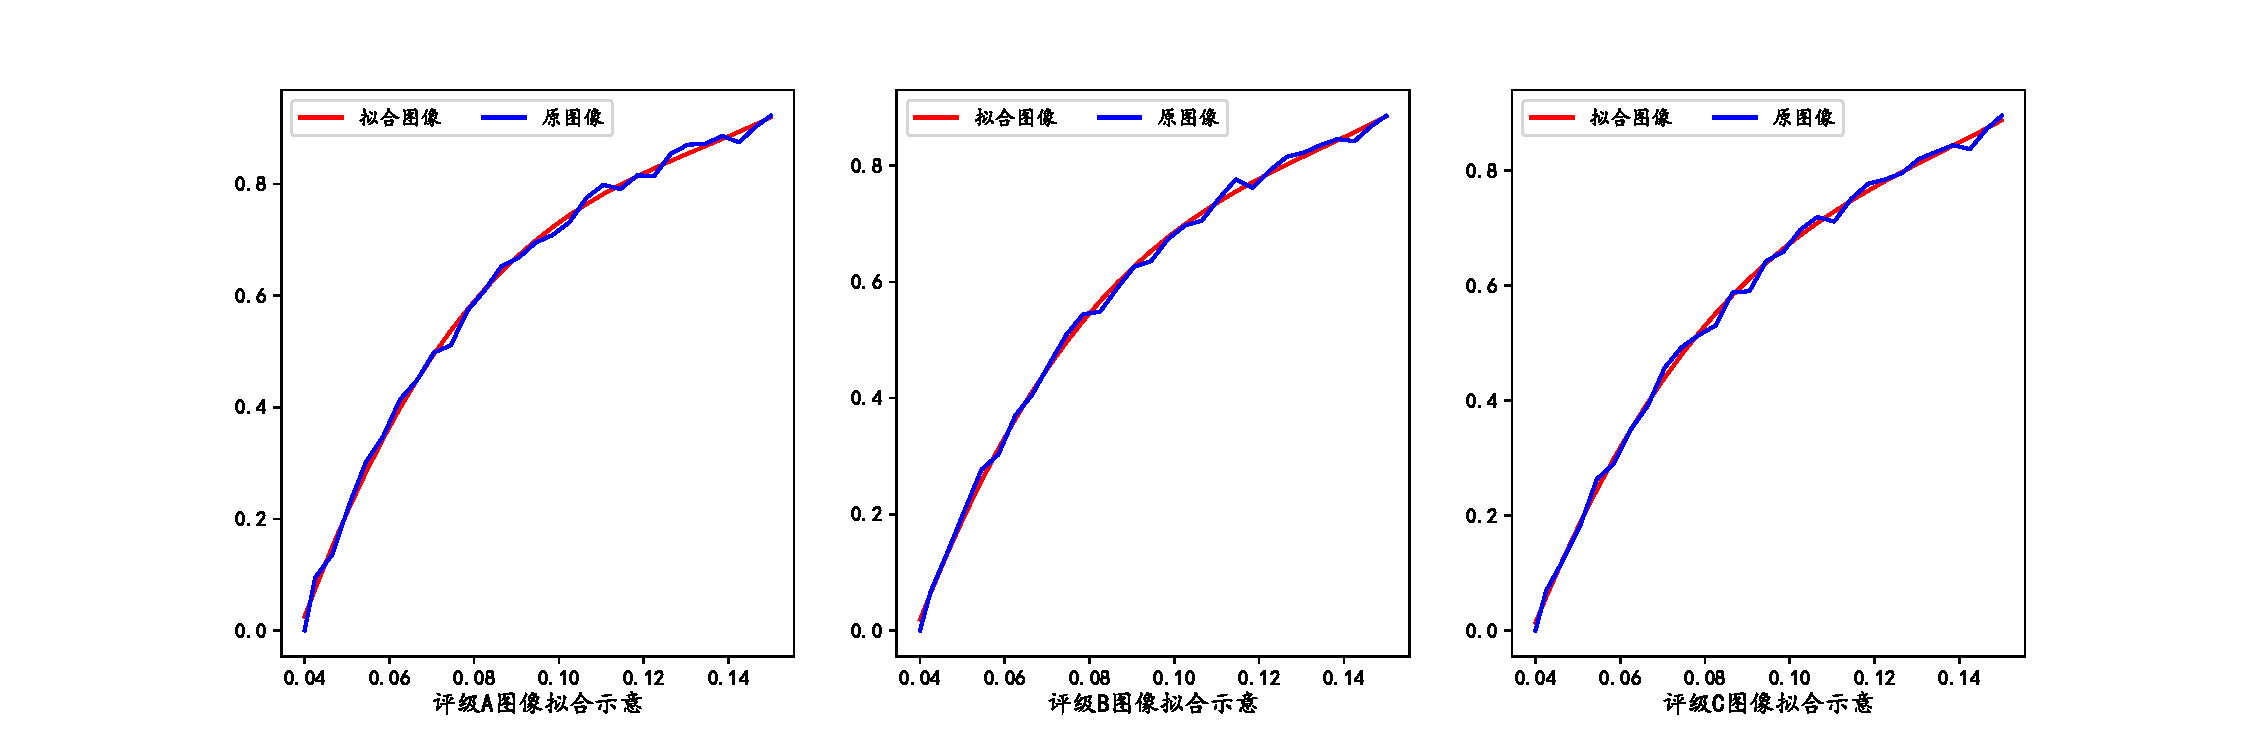
\includegraphics[width = 1.0\textwidth]{贷款年利率-客户流失率函数关系拟合.pdf}
            \caption{贷款年利率 -- 客户流失率 函数关系拟合}
            \label {图:贷款年利率 -- 客户流失率 函数关系拟合}
            \begin{align}
                S_A &= 640.9 \times x^3 - 258.6 \times x^2 + 37.97 \times x - 1.121 \\
                S_B &= 552.8 \times x^3 - 225.1 \times x^2 + 33.99 \times x - 1.017 \\
                S_C &= 504.7 \times x^3 - 207.4 \times x^2 + 32.16 \times x - 0.9735 
            \end{align}
        \end{figure}
        
        假定一个客户可以带来多个潜在客户,我们近似认为未来近三年内银行信贷客户每年以指数增长,以$a_{nj}$代表第$n$年该银行信誉评级为$j$的信贷客户数目,则得到递推关系式为:
        \begin{equation}
            a_{(n + 1) j} = e^n \times a_{n j} \times (1 - x)
        \end{equation}\par
        我们以公式(\ref{公式:银行盈利目标函数})为目标函数,求出$x \in[0.04, 0.15]$时的函数最大值所对应的$x$值。
        \begin{equation}
            SUM = {\sum_{i = 1}^{3} \sum_{j = A}^{C} a_{ij} \times (1 - S_j)^i}
            \label {公式:银行盈利目标函数}
        \end{equation}\par
        代入数据得到对应的$x$值为 0.04 ,即作为银行基准利率。 \par
        根据央行规定,我们设定最低上浮利率为 $0.5 \%$、最高上浮利率为 $2.0 \%$ 。对风险评级最低的企业予以最低上浮利率,风险评级最高的企业予以最高上浮利率,
        将其他风险评级的企业均匀散列在限定区间内,得到所有 123 家企业的信贷利率。(见附录 B )\par
        综合企业信贷额度百分比和信贷利率两项数据,即作为银行的信贷策略。

    \section{问题二的建模与求解}
    \subsection{企业信贷额度求解}
        延续问题一中建立的数学模型,将第二问相关的附件 2 中的数据代入,计算出各企业的信贷风险值和信贷风险等级(见附录 C )以及贷款额度百分比,然后将
        贷款额度百分比收束到题目要求的区间内,再归一化处理得到实际的信贷额度百分比。题目二中给出银行年度
        贷款总额为 1 亿元,用年度贷款总额乘以各企业贷款额度百分比得出各企业贷款额度\footnote{风险评级为 1 或 2 的企业不予放贷}。\par
        302 家企业信贷风险值和信贷风险评级散点图如下图 \ref{图:2-1}(具体数据见附录 D )
        \begin{figure}[H]
            \centering
            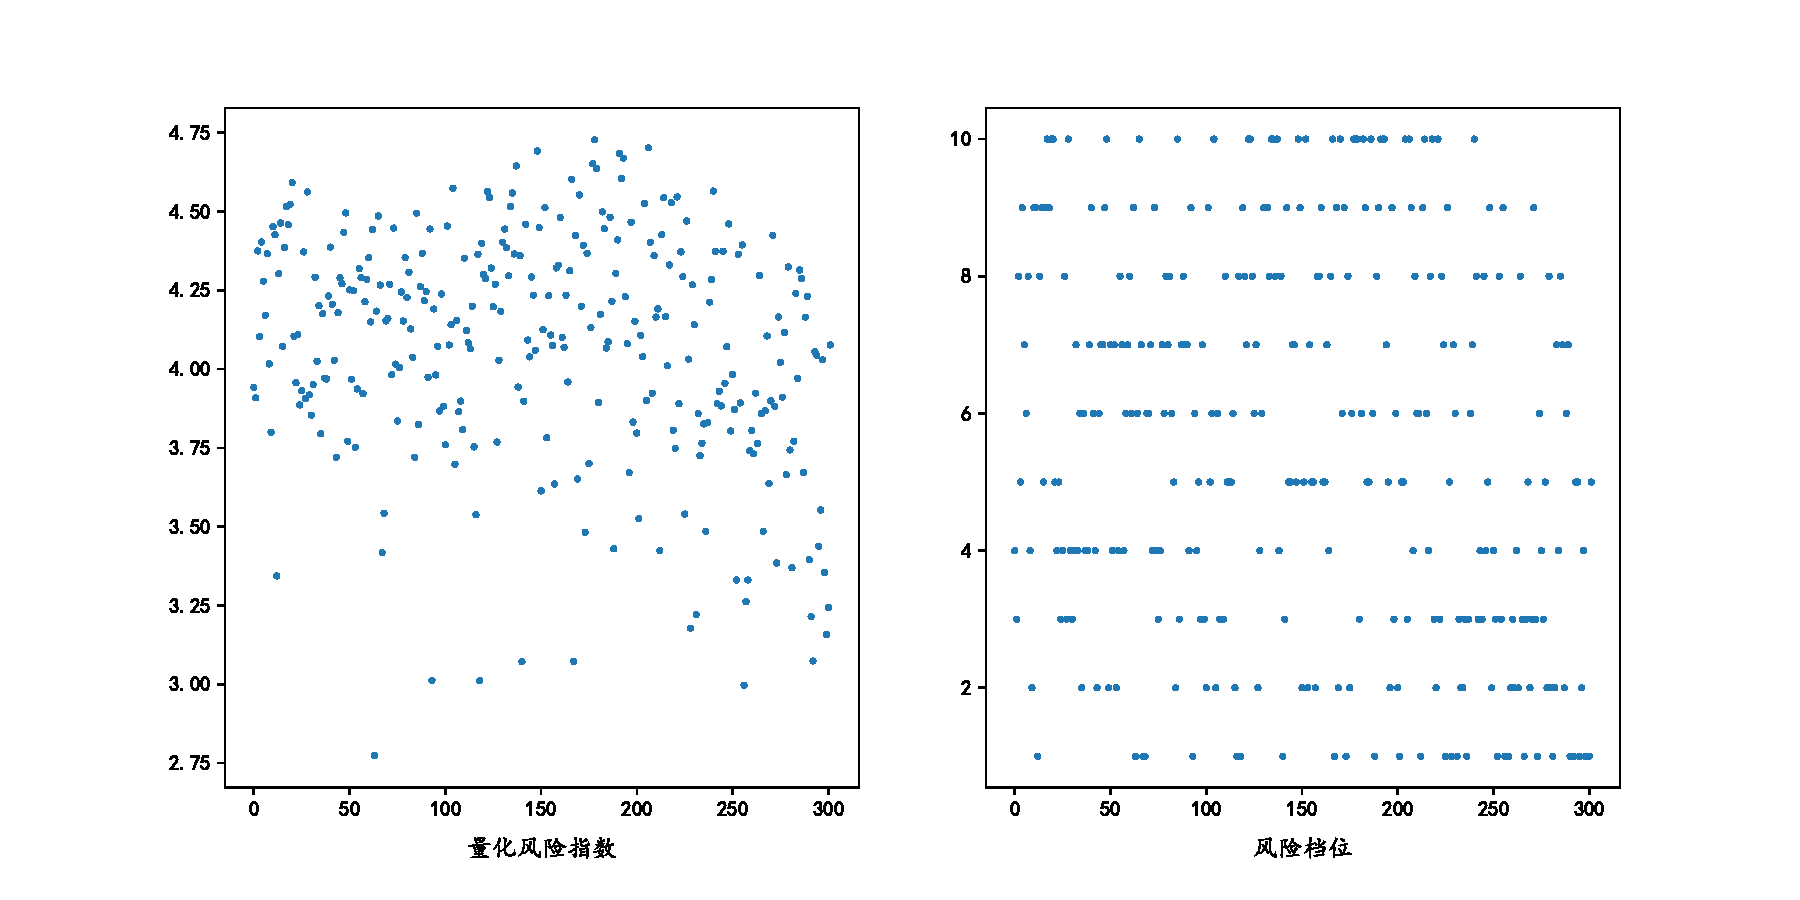
\includegraphics[width = 1.0\textwidth]{2_1.pdf}
            \caption{302 家企业信贷风险值和信贷风险评级}
            \label {图:2-1}
        \end{figure}
    \subsection{$RAROC$贷款定价模型理论基础}
        $RAROC$ \cite{doi:10.1111/j.1745-6622.1996.tb00117.x}原意是 $Risk - adjusted Return on Capital$,于二十世纪七十年代由美国信孚银行首创,最初的目的是为了度量银行信贷资产组合的风险,
        以及在特定损失率下为限制风险敞口所必须的权益资本。后来,由于$RAROC$克服了传统绩效考核的缺陷,逐渐成为银行进行风险管理和绩效考核方面的核心手段之一。
        如今,$RAROC$模型已成为当今国际银行业用于资本配置和贷款风险定价的核心技术手段。\par
        $RAROC$ 模型\cite{段翀2019}本质上是基于风险调整后的经济资本收益率,它将相关收费、运营成本、资金成本、预期损失、经济资本纳入考量指标,从而得到单位风险的利益最大化,
        确保贷款利率能够覆盖贷款项目的成本与风险。\par
        $RAROC$的基本计算公式为:
        \begin{equation*}
            \begin{split}
            RAROC &= \text{风险调整受益} \div \text{经济资本} \\
                  &= (\text{收入} - \text{成本费用} - \text{预期损失}) \div \text{经济资本} \\
                  &= (\text{贷款利息} + \text{贷款相关收费} - \text{运营成本} - \text{资金成本} - \text{预期损失}) \div \text{经济资本}
            \end{split}
        \end{equation*}\par
        其中,贷款利息是贷款额度、贷款利率与贷款期限三者的乘积。贷款额度($L$)、将贷款利率($r$)、贷款期限($T$)、贷款相关收费($IC$)、
        运营成本($OC$)、资金成本($DC$)、经济资本($EC$)、预期损失($EL$)全部代入$RAROC$公式并进行推导,得到贷款利率计算公式如下:
        \begin{equation}
            RAROC = \frac{(L \times r \times T + IC - OC - DC - EL)}{EC}
        \end{equation}
    \subsection{改进的$RAROC$模型}
        \begin{enumerate}
            \item \textbf{期限$T$}。本题银行贷款期限为 1 年,所以 $T = 1$。
            \item \textbf{贷款相关费用$IC$}。不考虑企业贷款时咨询费等额外费用,贷款时银行只收取贷款利息$L \times r \times T$,所以贷款相关收费为 0 $(IC = 0)$。
            \item \textbf{运营成本$OC$和资金成本$DC$}。由于题目中所给银行的名字信息不全,我们无法获取该银行的运营成本和资金成本。
                  因此,不妨认为该银行的运营成本和资金成本为除去无法收回贷款以外的其他损失,在本题中即为未来潜在客户流失所造成的经济损失。
                  给出计算公式:
                  \begin{equation}
                    \begin{split}
                      \text{运营成本和资金成本} &= \text{贷款额度} \times \text{贷款利率} \times \text{未来三年内客户相对流失率} \\
                        \iff OC + DC &= (L \times r \times \text{相对流失率}) 
                    \end{split}
                  \end{equation}
                  \begin{equation}
                      \text{某信誉等级的相对流失率} = \frac{\text{三年后客户实际数量}}{\text{流失率恒等于零的三年后客户数量}}
                  \end{equation}
                  \begin{equation}
                      \text{相对流失率} = \text{某信誉等级的相对流失率} \times \frac{\text{该信誉等级的公司数量}}{\text{总公司数}}
                  \end{equation}
            \item \textbf{预期损失$EL$}。
                  \begin{equation}
                    \begin{split}
                      \text{预期损失} &= sum [\text{风险暴露资金} \times \text{预期违约率} \times \text{违约流失率}] \\
                       \iff  EL      &= \sum_{i = 1}^{n = 302} EAD_i \times EDF_i \times LGD_i 
                    \end{split}
                  \end{equation} \par
                  每一项贷款所对应的公司信誉评级不同,则对应的预期违约率和违约流失率也不同,即 $EDF_i$ 和 $LGD_i$ 也不同。
                  \begin{enumerate}
                      \item $EAD$ 的值。
                            由于只考虑银行进行的贷款业务,但实际中银行业务种类繁多,所以每项贷款的风险暴露资金即为该项贷款额度乘以相关倍数
                            $(EAD_i = k \times L_i \times (1 + r), \ \text{其中\ } k = 18 )$。
                      \item $EDF$ 的值。
                            依据表 \ref{表:不同信用等级的一年后预期违约率} 国际信用评级穆迪投资服务有限公司的历史企业贷款数据统计结果:\par
                        \begin{table}[H]\begin{center}
                            \begin{tabular}{|c|c|c|}
                                \hline
                                序号 & 信用等级 & 预期违约率 $EDF$ \\
                                \hline
                                1   & $AA$ & $0 \%$ \\
                                2   & $A$  & $0.06 \%$ \\
                                3   & $BB$ & $0.09 \%$ \\
                                4   & $B$  & $0.15 \%$ \\
                                5   & $CC$ & $1.06 \%$ \\
                                6   & $C$  & $5.20 \%$ \\
                                7   & $DD$ & $7.63 \%$ \\
                                8   & $D$  & $12.16 \%$ \\ 
                                \hline                               
                            \end{tabular}
                            \caption{不同信用等级的一年后预期违约率}
                            \label {表:不同信用等级的一年后预期违约率}
                        \end{center}\end{table}
                        根据巴赛尔协议和模型所需,我们选取相应两档平均值作为
                        本模型 $A$、$B$、$C$、$D$ 四挡的 $EDF$ 值。求得:
                        \[
                            EDF_A = 0.03 \% \quad EDF_B = 0.12 \% \quad EDF_C = 3.13 \% \quad EDF_D = 9.89 \%
                        \] \par
                        \item $LGD$ 的值。
                          著名的信用评级机构穆迪公司的 $Carty$ 和 $Liberman$ 通过长期研究给出了不同偿付优先等级和
                          不同信用等级借款人的违约损失率,如表 \ref{表:不同信用等级借款人的违约损失率} :
                          \begin{table}[H]
                              \begin{center} \begin{tabular}{>{\centering}p{6em}>{\centering\arraybackslash}p{10em}}
                                  \hline
                                  信用等级 & 违约损失率 \\
                                  \hline
                                  $A$     & $8 \%$  \\
                                  $B$     & $24 \%$  \\
                                  $C$     & $36 \%$  \\
                                  $D$     & $43 \%$  \\
                                  \hline
                              \end{tabular}
                              \caption{不同信用等级借款人的违约损失率$(LGD)$}
                              \label {表:不同信用等级借款人的违约损失率}
                              \end{center}
                          \end{table}
                \end{enumerate}\par
            \item \textbf{$EC$ 的值}。
                经济资本指的是用于承担业务风险或购买外来收益的股东投资总额,
                是用来承担非预期损失和保持正常经营所需的资本,是银行所承担风险的最低要求。
                我们假定本题中银行给中小企业的贷款类型只有一种类型,结合本题我们认为该贷款类型为现实中的企业流动资金贷款,
                根据建设银行《经济资本预算管理暂行办法》,企业流动资金贷款额度为经济资本的
                $10 \%$ 左右 $(EC \times 10 \% = L)$。
        \end{enumerate}
    \subsection{运用改进后的 $RAROC$ 模型计算贷款利率}
        以不良贷款率低于 $ 5 \%$ 为约束\footnote{不良贷款率指贷款违约的预期损失 $(EL)$ 与贷款总额 $(L)$ 的比值。},以 $RAROC$ 函数
        为目标函数,求出目标函数的最大值为 $ 6.65 \%$ ,作为银行信贷基准利率。再根据风险评级对各企业实际贷款利率予以不同程度上浮,得到所有 302 家
        企业的信贷利率。\par
        302 家企业信贷额度百分比和信贷利率散点图如下图 \ref{图:2-2}(具体数据见附录 D ) :
        \begin{figure}[H]
            \centering
            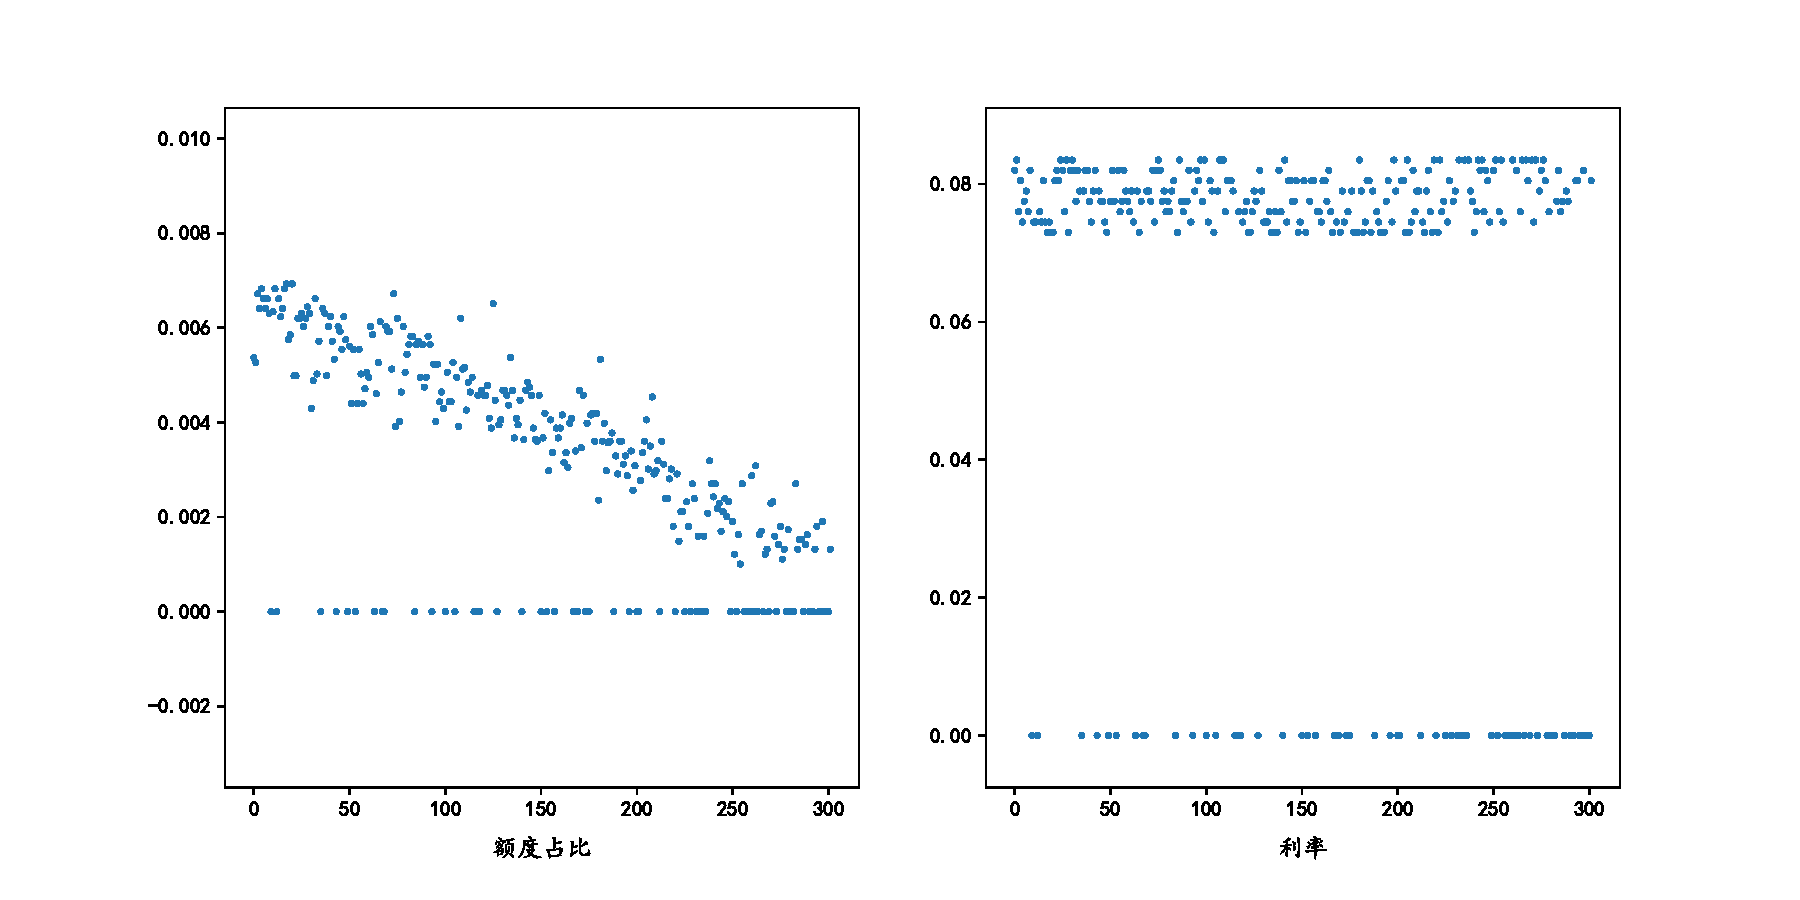
\includegraphics[width = 1.0\textwidth]{2_2.pdf}
            \caption{302 家企业信贷额度百分比和信贷利率}
            \label {图:2-2}
        \end{figure}
    
    \section{问题三的建模与求解}
        今年上半年我国受新冠疫情影响,中小微企业破产率急剧上升,中国政府迅速出台相关政策放宽贷款要求,
        通过降低基准贷款利率等措施,救活了许多受到疫情冲击的中小微企业。因此,针对第三问中问及的可能突发因素的影响,
        我们主要讨论研究``新冠病毒疫情''对各企业的影响和银行相应的信贷调整策略,最后也给出了部分其他突发情况的讨论与研究。
    \subsection{新冠疫情影响下的我国现状分析}
        我们根据企业类型对附件 2 中的 302 家企业进行分类汇总,如图 \ref{图:各类型企业频数} :
        \begin{figure}[H]
            \centering
            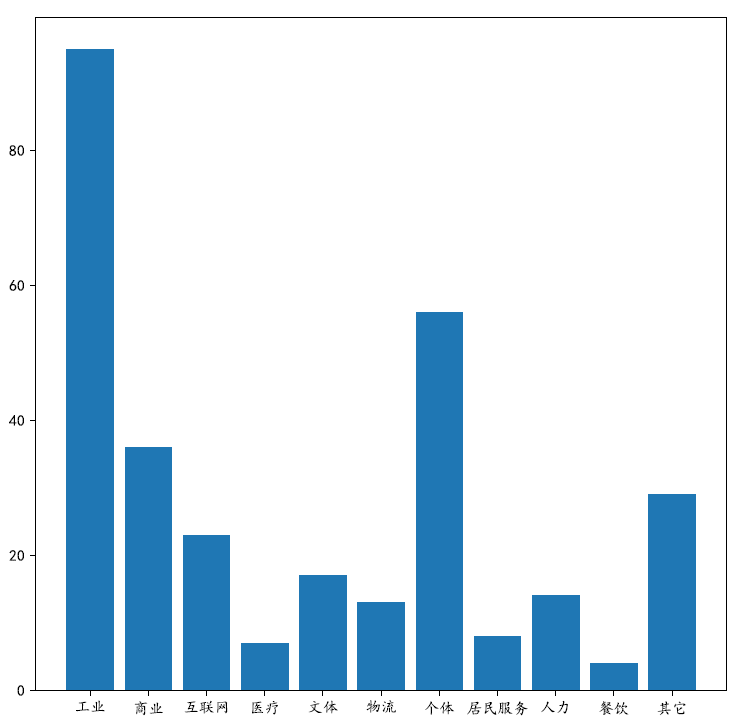
\includegraphics[width = 0.8\textwidth, height = 0.4\textheight]{第三问企业分类柱形图.png}
            \caption{各类型企业频数}
            \label {图:各类型企业频数}
        \end{figure}
        \begin{enumerate}
            \item \textbf{工业、商业、人力 } \par
                  对于该类\textbf{劳动力密集型企业},受到损失较大。一方面,因为疫情原因企业员工无法回到工作岗位上,企业无法复工复产,从而无法
                  创造受益。另一方面,企业还需承担员工的基本工资、场地和机器等租赁费用,企业的支出依旧保持较高水平。
            \item \textbf{文体、居民服务、餐饮} \par
                  对于该类\textbf{服务型企业},受到损失较大。疫情期间人们出行活动受阻,服务行业几乎失去了服务对象,所以企业受益严重下滑。
            \item \textbf{医疗、物流 } \par
                  对于该类\textbf{受政策影响较大的企业},企业收益有较大幅度增长。
                  医疗行业是我国抵御新冠疫情的关键行业,而物流行业则是保障我们在出行不便时基本生活状况的支撑行业,在新冠疫情期间及未来很长一段时间内,
                  国家都会重点扶持这类行业。在政策倾斜和市场环境的双重影响下,疫情带来的损失几乎可以忽略不计,而这类行业往往还能够有所盈利。
            \item \textbf{个体户}\par
                  对于 \textbf{个体户}而言,受到的损失较小。个体户负债率相对较低甚至无负债,所以在疫情期间相较于其他高负债率企业的经济风险更小。
                  同时个体户的财政收支更为灵活,人工费用微乎其微,可以在一定程度上减缓支出,从而达到维持收支平衡的效果。
            \item \textbf{互联网企业}\par
                  对于该类\textbf{劳动力离散型企业},企业收益有较小幅度增长。
                  互联网企业充分利用互联网的优势,实现远程办公,所以企业的正常运作基本不受影响,且公司在食堂、交通等方面的支出极大程度上减少,
                  从而使得企业支出有所下降。
            \item \textbf{其他行业}\par
                  对于 \textbf{其他行业},因无法评估疫情对其造成的影响,且该类企业数量较少,所以我们认为这些企业的发展
                  现状与疫情影响相关性较低。
        \end{enumerate}
    \subsection{我国行业的未来发展分析}
        \begin{enumerate}
            \item 对于\textbf{工业、文体、居民服务、餐饮}来说,由于突然爆发的新冠疫情导致的企业利益受损会随着后疫情时代的到来而得到缓解。
                  一方面,新冠疫情缓解之后,人们的生活封闭状况会逐步放开,人们复工复产积极性大幅提升,所以初步预测工业企业的发展潜力较高。
                  另一方面,人们娱乐消费支出逐步反弹回升,有利于文体、居民服务和餐饮业的回暖,所以我们初步预测这些行业未来发展潜力良好。
            \item 对于\textbf{医疗、物流}行业,即使进入后疫情时代,国家政策的扶持力度短时间内不会减弱,人们对于医疗、物流行业的依赖程度短期内不会下降,
                  该类行业很可能会保持疫情期间的水平。此外,疫情的冲击激发了人们对医疗、物流行业的重视程度,企业的受益将会得到持续增长,所以我们能够预测其未来发展潜力良好。
            \item 对于\textbf{互联网企业},疫情期间所受到的损失较小,充分印证了互联网企业在支出方面一定程度上的缩减不会影响企业发展。同时
                  人们对于互联网的依赖程度的上升说明互联网在日常生活中的不可替代性,这些都为互联网企业未来发展奠定良好基础,所以可以认为互联网企业的发展潜力会保持较好的势头。
            \item 对于\textbf{个体户},因为其规模较小,在出现负收益时缺乏足够的抵御风险资金,导致个体户的发展前景较为黯淡。
            \item 对于\textbf{商业},一方面人们因为疫情的居家隔离政策导致后疫情时代的消费意愿会明显上升,另一方面人们在疫情期间的商业消费减少,综合考量后,我们
                  认为商业的发展水平会反弹至疫情前的水平,但很难逾越该水平,所以我们认为商业的发展前景一般。
            \item 对于\textbf{其他行业},因企业数量较少且无法评估疫情对其造成的影响,所以我们认为这些企业的未来发展前景相对疫情前不变。
        \end{enumerate}
    \subsection{新冠疫情影响下的银行信贷调整策略}
        在问题二中,我们通过给企业年收入、年利润和信誉评级赋权重来确定贷款额度。经过上述分析与优化,现在我们基于企业现状来调整年收入档次,增加企业发展前景指标,以年收入、年利润
        、信誉评级和发展前景四个指标去衡量贷款额度。分析权威资料后,我们得出四个指标所占权重分别为$0.6$、$0.1$、$0.1$、$0.2$,计算得到各企业在新冠疫情影响后的贷款额度百分比。(见附件 E )\par
        我们沿用 $RAROC$ 模型去确定银行信贷基准利率,再根据企业信誉评级进行奖惩。同时根据国家扶持政策,所有企业的贷款利率均降低两个档次,其中医疗、物流行业的利率再降低四个档次,工业再降低二个档次,
        计算并汇总得出各企业在新冠疫情影响下的实际信贷利率。(见附件 E )\par
        信贷策略调整前后,各企业贷款额度百分比及贷款利率对比,如图 \ref{图:贷款额度百分比分布对比} 、图 \ref{图:贷款利率分布对比} :
        \begin{figure}[H]
            \centering
            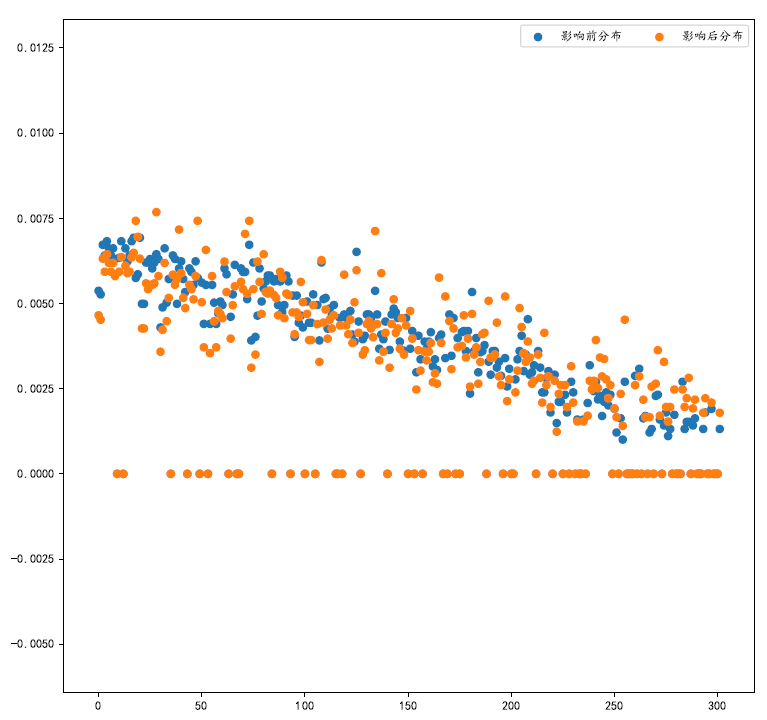
\includegraphics[width = 0.6 \textwidth]{com_1.png}
            \caption{贷款额度百分比分布对比}
            \label {图:贷款额度百分比分布对比}
        \end{figure}
        \begin{figure}[H]
            \centering
            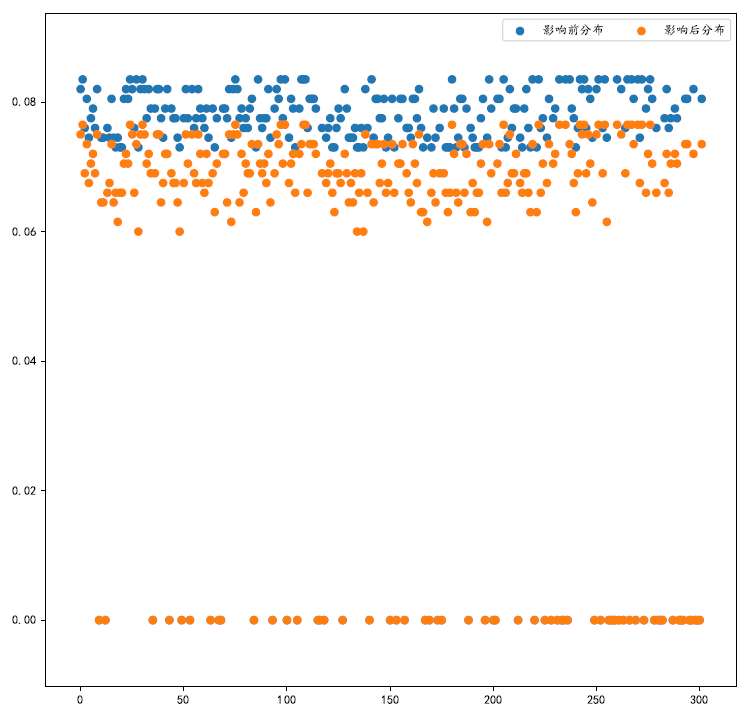
\includegraphics[width = 0.6 \textwidth]{com_2.png}
            \caption{贷款利率分布对比}
            \label {图:贷款利率分布对比}
        \end{figure}
    
    \subsection{其他突发因素影响下的银行信贷调整策略(以科研突破为例)}
    假定突发情况为某一领域科研突破,科研产品迅速投入市场。
        \begin{enumerate}
            \item 若该领域为工业领域的机器生产,则可以使得以机器生产、使用为主的企业类型成本大幅度降低,比如工业、医疗企业。
                我们将工业、医疗企业的年利润指标提高三个档次,再进行后续计算。
            \item 而对于劳动力支撑型企业也可以在一定程度上降低人工成本费,例如物流、人力成本。
                我们可以将物流、人力的年利润指标提高一个档次,再进行相关计算。
            \item 若该领域为互联网领域技术的突破,则可以使得互联网相关企业的年收入、年利润指标均增加四档,再重新计算。
            \item 而对于与互联网结合程度较紧密的企业类型,比如工业、商业、医疗、物流企业,均可以根据具体实际情况即互联网技术对于企业生产运营的实际作用,提高上述企业一到二个档次来进行后续计算。
        \end{enumerate}
    若该领域为交通领域新能源的突破,则可以使得交通运输成本较高的企业成本得到降低,例如物流,我们可以将物流的年利润指标提高两个档次,再去用问题二中的模型进行贷款额度、贷款利率的计算,而交通运输成本的降低则会导致人力类型企业的单位成本相对升高我们可以将人力类型企业年收入、年利润指标均降低两个档次,再进行贷款额度和贷款利率的重新计算。
    
    \section{模型的评价}
    \subsection{模型优点}
    \begin{enumerate}
        \item $ANP$ 网络结构能够很好反映现实中系统中各元素存在的依赖和反馈关系,通过运用 $ANP$ 网络结构我们能够精准
                得到该系统中各元素对系统的权重占比。
        \item 灰色系统理论直接对原始数据进行统计整理,具有可靠性强、推广性高和结果高度客观等优点。        
        \item $RAROC$ 贷款定价模型克服了传统模式的缺陷,有效减少人为的主观性影响,可以衡量商业银行在长期内
             的实际业务业绩和承担的风险,使货款定价更客观合理。
    \end{enumerate}
    \subsection{模型缺点}
    \begin{enumerate}
        \item 在实际大型应用中,由于信贷风险评估的系统复杂度,很难运用 $ANP$ 网络结构来划分层次。
        \item 影响中小微企业信贷评估的指标错综复杂,本文值采用了具有代表性的九个指标,指标体系可能存在一定的欠完整性。
        \item $RAROC$ 贷款定价模型中涉及到的预期违约率 $(EDF)$ 和违约损失率 $(LGD)$ 都采用了国际统计数据,忽略了国内社会环境所可能导致的数值上的偏差,
              对于我国银行贷款策略的指导上可能存在一定的误差。
    \end{enumerate}
    
    \bibliographystyle{plain}  % 参考文献
    \bibliography{ref}
    
    \newpage
    \appendix
    {\Large\textbf{附录}}\par
    \textbf{支撑文件汇总}
    \begin{enumerate}
        \item 1-1.pdf
        \item 1-2.pdf
        \item 2-1.pdf
        \item 2.2.pdf
        \item 流程图.pdf
        \item 贷款年利率-客户流失率函数关系拟合.pdf
        \item 第三问企业分类柱形图.png
        \item 风险评价网络层次图.png
        \item $com\_1$.png
        \item $com\_2$.png
        \item 123家企业风险量化值和风险评级.csv
        \item 123家企业信贷额度百分比和信贷利率.csv
        \item 302家企业风险量化值和风险评级.csv
        \item 302家企业信贷额度百分比和信贷利率.csv
        \item 第三题信贷额度百分比和信贷利率.csv
        \item code.rar
    \end{enumerate}
    
    \section{ 123 家企业风险量化值和风险评级} 
    \begin{longtable}{>{\centering}p{6em}>{\centering\arraybackslash}p{20em}>{\centering\arraybackslash}p{10em}}
            \hline
            ID	&风险量化值 	&风险评级 \\
            \hline
            E1	&3.602988408	&2	\\
            E2	&4.504703214	&10	\\
            E3	&4.34497938	    &9	\\
            E4	&4.222552397	&7	\\
            E5	&4.119119741	&5	\\
            E6	&4.337403357	&8	\\
            E7	&4.392146977	&9	\\
            E8	&4.051002123	&5	\\
            E9	&4.325244788	&8	\\
            E10	&4.176027041	&6	\\
            E11	&3.988987068	&4	\\
            E12	&4.272760462	&8	\\
            E13	&4.051002123	&5	\\
            E14	&4.343812301	&9	\\
            E15	&3.979841772	&4	\\
            E16	&4.416012685	&9	\\
            E17	&4.286241841	&8	\\
            E18	&4.248396165	&8	\\
            E19	&3.865895364	&3	\\
            E20	&3.575459425	&2	\\
            E21	&3.984768257	&4	\\
            E22	&4.400400251	&9	\\
            E23	&4.088270205	&5	\\
            E24	&4.545840614	&10	\\
            E25	&4.596881814	&10	\\
            E26	&3.936924862	&4	\\
            E27	&4.251854253	&8	\\
            E28	&3.959293382	&4	\\
            E29	&3.982976952	&4	\\
            E30	&4.23632341	    &8	\\
            \hline\hline
            E31	&4.393372447	&9	\\
            E32	&4.588117655	&10	\\
            E33	&3.949183688	&4	\\
            E34	&4.215799283	&7	\\
            E35	&4.314527828	&8	\\
            E36	&4.407743283	&9	\\
            E37	&4.019795275	&4	\\
            E38	&4.187429333	&6	\\
            E39	&4.175355122	&6	\\
            E40	&4.640836311	&10	\\
            E41	&4.666984883	&10	\\
            E42	&3.827760022	&3	\\
            E43	&4.123227992	&5	\\
            E44	&4.194817424	&7	\\
            E45	&3.751379363	&3	\\
            E46	&4.185749472	&6	\\
            E47	&4.177636246	&6	\\
            E48	&4.71415248	    &10	\\
            E49	&4.099283695	&5	\\
            E50	&4.200231058	&7	\\
            E51	&4.422176319	&9	\\
            E52	&3.936036621	&3	\\
            E53	&4.169219018	&6	\\
            E54	&4.480882539	&10	\\
            E55	&4.383565969	&9	\\
            E56	&4.136537268	&6	\\
            E57	&3.841204892	&3	\\
            E58	&4.527858119	&10	\\
            E59	&4.117078511	&5	\\
            E60	&4.226306657	&7	\\
            E61	&4.590346023	&10	\\
            E62	&4.301276879	&8	\\
            E63	&4.23083531	    &7	\\
            E64	&4.232679489	&7	\\
            \hline\hline
            E65	&4.260092745	&8	\\
            E66	&3.495111014	&2	\\
            E67	&4.554423752	&10	\\
            E68	&3.4826737	    &1	\\
            E69	&3.618119483	&2	\\
            E70	&4.202043734	&7	\\
            E71	&4.213862916	&7	\\
            E72	&3.976411563	&4	\\
            E73	&4.571402485	&10	\\
            E74	&3.864656559	&3	\\
            E75	&3.962780407	&4	\\
            E76	&4.338036698	&8	\\
            E77	&3.793241808	&3	\\
            E78	&4.211112226	&7	\\
            E79	&4.100674057	&5	\\
            E80	&4.144424828	&6	\\
            E81	&4.220797606	&7	\\
            E82	&3.871180195	&3	\\
            E83	&3.743631225	&2	\\
            E84	&4.208674731	&7	\\
            E85	&4.475004284	&10	\\
            E86	&3.604281681	&2	\\
            E87	&4.321009408	&8	\\
            E88	&4.47619182	    &10	\\
            E89	&3.174215826	&1	\\
            E90	&4.403643059	&9	\\
            E91	&4.166300128	&6	\\
            E92	&4.131101389	&6	\\
            E93	&4.121696424	&5	\\
            E94	&3.4714942	    &1	\\
            E95	&4.0907802	    &5	\\
            E96	&3.352404095	&1	\\
            E97	&4.462041337	&9	\\
            E98	&4.165989579	&6	\\
            \hline\hline
            E99	&3.983392949	&4	\\
            E100	&4.371661397	&9	\\
            E101	&3.882752964	&3	\\
            E102	&3.573057494	&2	\\
            E103	&4.150587935	&6	\\
            E104	&3.442097249	&1	\\
            E105	&3.742991301	&2	\\
            E106	&4.128302015	&5	\\
            E107	&2.946920076	&1	\\
            E108	&4.029024595	&4	\\
            E109	&3.85880339	    &3	\\
            E110	&3.745691932	&2	\\
            E111	&3.698309306	&2	\\
            E112	&4.093284886	&5	\\
            E113	&3.814777348	&3	\\
            E114	&3.284189375	&1	\\
            E115	&3.013395539	&1	\\
            E116	&3.602265413	&2	\\
            E117	&3.766987164	&3	\\
            E118	&3.216294467	&1	\\
            E119	&3.312907565	&1	\\
            E120	&3.704638685	&2	\\
            E121	&3.435906181	&1	\\
            E122	&3.284189375	&1	\\
            E123	&3.468567078	&1	\\
            \hline
    \end{longtable}\newpage

    \section{ 123 家企业信贷额度百分比和信贷利率} 
    \begin{longtable}{>{\centering}p{6em}>{\centering\arraybackslash}p{20em}>{\centering\arraybackslash}p{10em}}
        \hline
        ID	&信贷额度百分比	  &信贷利率	\\
        \hline
        E1	&0.012410461	&0.016658337	\\
        E2	&0.016658337	&0.016408462	\\
        E3	&0.016408462	&0.015908712	\\
        E4	&0.015908712	&0.013160087	\\
        E5	&0.013160087	&0.015908712	\\
        E6	&0.015908712	&0.016408462	\\
        E7	&0.016408462	&0.015408962	\\
        E8	&0.015408962	&0.016158587	\\
        E9	&0.016158587	&0.015658837	\\
        E10	&0.015658837	&0.014659337	\\
        E11	&0.014659337	&0.016158587	\\
        E12	&0.016158587	&0.014242879	\\
        E13	&0.014242879	&0.015242379	\\
        E14	&0.015242379	&0.015159087	\\
        E15	&0.015159087	&0.016408462	\\
        E16	&0.016408462	&0.014242879	\\
        E17	&0.014242879	&0.014742629	\\
        E18	&0.014742629	&0.011494253	\\
        E19	&0.011494253	&0.011244378	\\
        E20	&0.011244378	&0.011744128	\\
        E21	&0.011744128	&0.014992504	\\
        E22	&0.014992504	&0.011994003	\\
        E23	&0.011994003	&0.015242379	\\
        E24	&0.015242379	&0.012660336	\\
        E25	&0.012660336	&0.009411961	\\
        E26	&0.009411961	&0.010411461	\\
        E27	&0.010411461	&0.01282692	\\
        E28	&0.01282692	    &0	\\
        E29	&0	            &0.014742629	\\
        E30	&0.014742629	&0.012660336	\\
        E31	&0.012660336	&0.014076295	\\
        E32	&0.014076295	&0.010827919	\\
        \hline\hline
        E33	&0.010827919	&0.01332667	\\
        E34	&0.01332667	    &0.009995002	\\
        E35	&0.009995002	&0	\\
        E36	&0	            &0.009411961	\\
        E37	&0.009411961	&0.013076795	\\
        E38	&0.013076795	&0.011910711	\\
        E39	&0.011910711	&0.012660336	\\
        E40	&0.012660336	&0.011494253	\\
        E41	&0.011494253	&0.01232717	\\
        E42	&0.01232717	    &0.012577045	\\
        E43	&0.012577045	&0.009245377	\\
        E44	&0.009245377	&0	\\
        E45	&0	            &0.01232717	\\
        E46	&0.01232717	    &0.01182742	\\
        E47	&0.01182742	    &0.01382642	\\
        E48	&0.01382642	    &0.011410961	\\
        E49	&0.011410961	&0.01332667	\\
        E50	&0.01332667	    &0.010744628	\\
        E51	&0.010744628    &0	\\
        E52	&0	            &0.011161086	\\
        E53	&0.011161086	&0.011494253	\\
        E54	&0.011494253	&0.011244378	\\
        E55	&0.011244378	&0.008995502	\\
        E56	&0.008995502	&0.009411961	\\
        E57	&0.009411961	&0.011494253	\\
        E58	&0.011494253	&0.009745127	\\
        E59	&0.009745127	&0.009078794	\\
        E60	&0.009078794	&0.010328169	\\
        E61	&0.010328169	&0.009578544	\\
        E62	&0.009578544	&0.01282692	\\
        E63	&0.01282692	    &0.009328669	\\
        E64	&0.009328669	&0.00791271	\\
        E65	&0.00791271	    &0.005663835	\\
        E66	&0.005663835	&0.010078294	\\
        \hline\hline
        E67	&0.010078294	&0.008995502	\\
        E68	&0.008995502	&0.00641346	\\
        E69	&0.00641346	    &0.009078794	\\
        E70	&0.009078794	&0.010494753	\\
        E71	&0.010494753	&0.008329169	\\
        E72	&0.008329169	&0.008662335	\\
        E73	&0.008662335	&0.00691321	\\
        E74	&0.00691321	    &0.00691321	\\
        E75	&0.00691321	    &0.006746627	\\
        E76	&0.006746627	&0.008329169	\\
        E77	&0.008329169	&0.009328669	\\
        E78	&0.009328669	&0.00691321	\\
        E79	&0.00691321	    &0.009328669	\\
        E80	&0.009328669	&0.005997001	\\
        E81	&0.005997001	&0	\\
        E82	&0	            &0.00541396	\\
        E83	&0.00541396	    &0.00791271	\\
        E84	&0.00791271	    &0.007246377	\\
        E85	&0.007246377	&0.00541396	\\
        E86	&0.00541396	    &0	\\
        E87	&0	            &0.007246377	\\
        E88	&0.007246377	&0.003998001	\\
        E89	&0.003998001	&0.006996502	\\
        E90	&0.006996502	&0.004581043	\\
        E91	&0.004581043	&0.00791271	\\
        E92	&0.00791271	    &0.004581043	\\
        E93	&0.004581043	&0.003331667	\\
        E94	&0.003331667	&0.004830918	\\
        E95	&0.004830918	&0.007079793	\\
        E96	&0.007079793	&0.005580543	\\
        E97	&0.005580543	&0.004830918	\\
        E98	&0.004830918	&0	\\
        E99	&0	            &0	\\
        E100	&0	        &0	\\
        \hline\hline
        E101	&0	        &0	\\   
        E102	&0	        &0	\\
        E103	&0	            &0.003831418	\\
        E104	&0.003831418	&0.004081293	\\
        E105	&0.004081293	&0.003165084	\\
        E106	&0.003165084	&0	\\
        E107	&0	            &0	\\
        E108	&0	            &0	\\
        E109	&0	            &0.002415459	\\
        E110	&0.002415459	&0	\\
        E111	&0	&0	\\
        E112	&0	&0	\\
        E113	&0	&0	\\
        E114	&0	&0	\\
        E115	&0	&0	\\
        E116	&0	&0	\\
        E117	&0	&0	\\
        E118	&0	&0	\\
        E119	&0	&0	\\
        E120	&0	&0	\\
        E121	&0	&0	\\
        E122	&0	&0	\\
        E123	&0	&0	\\
        \hline
    \end{longtable}\newpage
    
    \section{ 302 家企业风险量化值和风险评级} 
    \begin{longtable}{>{\centering}p{6em}>{\centering\arraybackslash}p{20em}>{\centering\arraybackslash}p{10em}}
        \hline
        ID	    &企业风险量化值	 &企业风险评级	\\
        \hline
        E124	&3.941743773	&4	\\
        E125	&3.908558848	&3	\\
        E126	&4.374486754	&8	\\
        E127	&4.10264723	    &5	\\
        E128	&4.402911619	&9	\\
        E129	&4.278627387	&7	\\
        E130	&4.170678502	&6	\\
        E131	&4.366003318	&8	\\
        E132	&4.016326949	&4	\\
        E133	&3.799523593	&2	\\
        E134	&4.451552529	&9	\\
        E135	&4.425861701	&9	\\
        E136	&3.343731635	&1	\\
        E137	&4.302359954	&8	\\
        E138	&4.463248187	&9	\\
        E139	&4.072206773	&5	\\
        E140	&4.385217256	&9	\\
        E141	&4.514838051	&10	\\
        E142	&4.457840262	&9	\\
        E143	&4.521957355	&10	\\
        E144	&4.591048572	&10	\\
        E145	&4.103957846	&5	\\
        E146	&3.95654953	    &4	\\
        E147	&4.108905074	&5	\\
        E148	&3.885968281	&3	\\
        E149	&3.931636118	&4	\\
        E150	&4.371469916	&8	\\
        E151	&3.906815294	&3	\\
        E152	&4.561694362	&10	\\
        E153	&3.918246463	&4	\\
        E154	&3.853834124	&3	\\
        E155	&3.950636492	&4	\\
        \hline\hline
        E156	&4.291492297	&7	\\
        E157	&4.025063322	&4	\\
        E158	&4.200556016	&6	\\
        E159	&3.794664068	&2	\\
        E160	&4.175447656	&6	\\
        E161	&3.970990128	&4	\\
        E162	&3.968503779	&4	\\
        E163	&4.231446469	&7	\\
        E164	&4.386724016	&9	\\
        E165	&4.205407135	&6	\\
        E166	&4.027530493	&4	\\
        E167	&3.720100313	&2	\\
        E168	&4.178601351	&6	\\
        E169	&4.289246846	&7	\\
        E170	&4.270281609	&7	\\
        E171	&4.433568639	&9	\\
        E172	&4.495129887	&10	\\
        E173	&3.770781685	&2	\\
        E174	&4.251000726	&7	\\
        E175	&3.96768167	    &4	\\
        E176	&4.248563394	&7	\\
        E177	&3.75149757	    &2	\\
        E178	&3.936710071	&4	\\
        E179	&4.318680205	&8	\\
        E180	&4.290236464	&7	\\
        E181	&3.921642156	&4	\\
        E182	&4.213534248	&6	\\
        E183	&4.284782497	&7	\\
        E184	&4.353258411	&8	\\
        E185	&4.149494293	&6	\\
        E186	&4.44302188	    &9	\\
        E187	&2.77382677	    &1	\\
        E188	&4.183720126	&6	\\
        E189	&4.485384965	&10	\\
        \hline\hline
        E190	&4.266207306	&7	\\
        E191	&3.417725783	&1	\\
        E192	&3.542280763	&1	\\
        E193	&4.152671782	&6	\\
        E194	&4.160831614	&6	\\
        E195	&4.268782087	&7	\\
        E196	&3.981710395	&4	\\
        E197	&4.44714435	    &9	\\
        E198	&4.015659809	&4	\\
        E199	&3.835271906	&3	\\
        E200	&4.004510725	&4	\\
        E201	&4.244283999	&7	\\
        E202	&4.152247005	&6	\\
        E203	&4.353104369	&8	\\
        E204	&4.227111136	&7	\\
        E205	&4.306934319	&8	\\
        E206	&4.127091725	&6	\\
        E207	&4.036975915	&5	\\
        E208	&3.720151738	&2	\\
        E209	&4.494220937	&10	\\
        E210	&3.823501547	&3	\\
        E211	&4.261121858	&7	\\
        E212	&4.36721476	    &8	\\
        E213	&4.216413215	&7	\\
        E214	&4.245690315	&7	\\
        E215	&3.97383579	    &4	\\
        E216	&4.444001188	&9	\\
        E217	&3.01222631	    &1	\\
        E218	&4.190413516	&6	\\
        E219	&3.981224568	&4	\\
        E220	&4.071983716	&5	\\
        E221	&3.867050132	&3	\\
        E222	&4.238031462	&7	\\
        E223	&3.881757005	&3	\\
        \hline\hline
        E224	&3.759626276	&2	\\
        E225	&4.453576492	&9	\\
        E226	&4.076195968	&5	\\
        E227	&4.140902079	&6	\\
        E228	&4.573467209	&10	\\
        E229	&3.698045457	&2	\\
        E230	&4.154290822	&6	\\
        E231	&3.86480008	    &3	\\
        E232	&3.898309166	&3	\\
        E233	&3.807545832	&3	\\
        E234	&4.351604915	&8	\\
        E235	&4.122114203	&5	\\
        E236	&4.083574049	&5	\\
        E237	&4.064377419	&5	\\
        E238	&4.199536174	&6	\\
        E239	&3.753089541	&2	\\
        E240	&3.537561088	&1	\\
        E241	&4.364139962	&8	\\
        E242	&3.011286616	&1	\\
        E243	&4.398401451	&9	\\
        E244	&4.300084347	&8	\\
        E245	&4.287269755	&7	\\
        E246	&4.563287267	&10	\\
        E247	&4.544464843	&10	\\
        E248	&4.320191946	&8	\\
        E249	&4.197153589	&6	\\
        E250	&4.269278208	&7	\\
        E251	&3.768445512	&2	\\
        E252	&4.028238415	&4	\\
        E253	&4.183114442	&6	\\
        E254	&4.402257051	&9	\\
        E255	&4.44403838	    &9	\\
        E256	&4.384480474	&9	\\
        E257	&4.295710772	&8	\\
        \hline\hline
        E258	&4.515777745	&10	\\
        E259	&4.558369109	&10	\\
        E260	&4.364988725	&8	\\
        E261	&4.644252075	&10	\\
        E262	&3.942812699	&4	\\
        E263	&4.359059445	&8	\\
        E264	&3.071982919	&1	\\
        E265	&3.898065714	&3	\\
        E266	&4.459215416	&9	\\
        E267	&4.091846689	&5	\\
        E268	&4.038494145	&5	\\
        E269	&4.291866425	&7	\\
        E270	&4.23407114	    &7	\\
        E271	&4.05920311	    &5	\\
        E272	&4.691531028	&10	\\
        E273	&4.448305953	&9	\\
        E274	&3.613456307	&2	\\
        E275	&4.124991461	&5	\\
        E276	&4.512240236	&10	\\
        E277	&3.781910112	&2	\\
        E278	&4.232157564	&7	\\
        E279	&4.107821105	&5	\\
        E280	&4.074846907	&5	\\
        E281	&3.635302459	&2	\\
        E282	&4.320615675	&8	\\
        E283	&4.328839585	&8	\\
        E284	&4.480446678	&9	\\
        E285	&4.100398252	&5	\\
        E286	&4.068719321	&5	\\
        E287	&4.234354293	&7	\\
        E288	&3.958865813	&4	\\
        E289	&4.311549065	&8	\\
        E290	&4.602003105	&10	\\
        E291	&3.072762508	&1	\\
        \hline\hline
        E292	&4.423967401	&9	\\
        E293	&3.65113625	    &2	\\
        E294	&4.551985412	&10	\\
        E295	&4.199359411	&6	\\
        E296	&4.392741669	&9	\\
        E297	&3.482407117	&1	\\
        E298	&4.366787332	&8	\\
        E299	&3.70004835	    &2	\\
        E300	&4.131244471	&6	\\
        E301	&4.651028578	&10	\\
        E302	&4.726870437	&10	\\
        E303	&4.635194162	&10	\\
        E304	&3.894171927	&3	\\
        E305	&4.173590808	&6	\\
        E306	&4.498426162	&10	\\
        E307	&4.445445596	&9	\\
        E308	&4.066528223	&5	\\
        E309	&4.086046319	&5	\\
        E310	&4.481349745	&10	\\
        E311	&4.214617345	&6	\\
        E312	&3.429921293	&1	\\
        E313	&4.303137949	&8	\\
        E314	&4.40957815	    &9	\\
        E315	&4.683322666	&10	\\
        E316	&4.604442882	&10	\\
        E317	&4.668581056	&10	\\
        E318	&4.229502362	&7	\\
        E319	&4.080570727	&5	\\
        E320	&3.671751633	&2	\\
        E321	&4.465952518	&9	\\
        E322	&3.831691255	&3	\\
        E323	&4.151189005	&6	\\
        E324	&3.796845277	&2	\\
        E325	&3.525768833	&1	\\
        \hline\hline
        E326	&4.107330733	&5	\\
        E327	&4.039123093	&5	\\
        E328	&4.524941468	&10	\\
        E329	&3.899923419	&3	\\
        E330	&4.701524201	&10	\\
        E331	&4.402336628	&9	\\
        E332	&3.923250625	&4	\\
        E333	&4.359880262	&8	\\
        E334	&4.164851221	&6	\\
        E335	&4.190661344	&6	\\
        E336	&3.424073053	&1	\\
        E337	&4.426203987	&9	\\
        E338	&4.543485802	&10	\\
        E339	&4.165915144	&6	\\
        E340	&4.010130436	&4	\\
        E341	&4.330058291	&8	\\
        E342	&4.52754523	    &10	\\
        E343	&3.806116018	&3	\\
        E344	&3.748079963	&2	\\
        E345	&4.545761513	&10	\\
        E346	&3.889885883	&3	\\
        E347	&4.371494959	&8	\\
        E348	&4.293325033	&7	\\
        E349	&3.539933765	&1	\\
        E350	&4.469504938	&9	\\
        E351	&4.031448329	&5	\\
        E352	&3.177894281	&1	\\
        E353	&4.266942096	&7	\\
        E354	&4.140421147	&6	\\
        E355	&3.221148084	&1	\\
        E356	&3.858647395	&3	\\
        E357	&3.725323146	&2	\\
        E358	&3.764373871	&2	\\
        E359	&3.826039766	&3	\\
        \hline\hline
        E360	&3.485008964	&1	\\
        E361	&3.830137821	&3	\\
        E362	&4.212205981	&6	\\
        E363	&4.283896683	&7	\\
        E364	&4.564403054	&10	\\
        E365	&4.373151626	&8	\\
        E366	&3.889746947	&3	\\
        E367	&3.929941541	&4	\\
        E368	&3.883032362	&3	\\
        E369	&4.373281318	&8	\\
        E370	&3.954467242	&4	\\
        E371	&4.070330722	&5	\\
        E372	&4.460359561	&9	\\
        E373	&3.803687127	&2	\\
        E374	&3.982502407	&4	\\
        E375	&3.871140023	&3	\\
        E376	&3.330854237	&1	\\
        E377	&4.36382754	    &8	\\
        E378	&3.892502506	&3	\\
        E379	&4.393673773	&9	\\
        E380	&2.996933994	&1	\\
        E381	&3.262258881	&1	\\
        E382	&3.330854237	&1	\\
        E383	&3.740478355	&2	\\
        E384	&3.805200589	&3	\\
        E385	&3.731044368	&2	\\
        E386	&3.923565471	&4	\\
        E387	&3.764373871	&2	\\
        E388	&4.296262191	&8	\\
        E389	&3.85828461	    &3	\\
        E390	&3.485008964	&1	\\
        E391	&3.867546544	&3	\\
        E392	&4.104835346	&5	\\
        E393	&3.63706953	    &2	\\
        \hline\hline
        E394	&3.898975642	&3	\\
        E395	&4.423907339	&9	\\
        E396	&3.881979634	&3	\\
        E397	&3.384712152	&1	\\
        E398	&4.165079087	&6	\\
        E399	&4.021458945	&4	\\
        E400	&3.910808651	&3	\\
        E401	&4.115909572	&5	\\
        E402	&3.664707272	&2	\\
        E403	&4.323780273	&8	\\
        E404	&3.743290046	&2	\\
        E405	&3.369940392	&1	\\
        E406	&3.770876691	&2	\\
        E407	&4.239769702	&7	\\
        E408	&3.970077367	&4	\\
        E409	&4.31410226	    &8	\\
        E410	&4.286587406	&7	\\
        E411	&3.67150825	    &2	\\
        E412	&4.164518916	&6	\\
        E413	&4.230226788	&7	\\
        E414	&3.39531581	    &1	\\
        E415	&3.21467294	    &1	\\
        E416	&3.074122003	&1	\\
        E417	&4.054356834	&5	\\
        E418	&4.04314201	    &5	\\
        E419	&3.437510393	&1	\\
        E420	&3.552882855	&2	\\
        E421	&4.029071582	&4	\\
        E422	&3.354044476	&1	\\
        E423	&3.157969841	&1	\\
        E424	&3.243692374	&1	\\
        E425	&4.076480118	&5	\\
        \hline
    \end{longtable}\newpage

    \section{ 302 家企业信贷额度百分比和信贷利率} 
    \begin{longtable}{>{\centering}p{6em}>{\centering\arraybackslash}p{11em}>{\centering\arraybackslash}p{11em}>{\centering\arraybackslash}p{6em}}
        \hline
        ID	    &信贷额度百分比	 &信贷额度(万元)	&信贷利率	\\
        \hline
        E124	&0.005369825	&53.69825048	&0.082	\\
        E125	&0.005265893	&52.6589295	    &0.0835	\\
        E126	&0.006720942	&67.20942318	&0.076	\\
        E127	&0.006409146	&64.09146025	&0.0805	\\
        E128	&0.006824874	&68.24874415	&0.0745	\\
        E129	&0.00661701	    &66.1701022	    &0.0775	\\
        E130	&0.006409146	&64.09146025	&0.079	\\
        E131	&0.00661701	    &66.1701022	    &0.076	\\
        E132	&0.006305214	&63.05213927	&0.082	\\
        E133	&0	            &0	            &0	\\
        E134	&0.006339858	&63.39857959	&0.0745	\\
        E135	&0.006824874	&68.24874415	&0.0745	\\
        E136	&0	            &0	            &0	\\
        E137	&0.00661701	    &66.1701022	    &0.076	\\
        E138	&0.006235926	&62.35925862	&0.0745	\\
        E139	&0.006409146	&64.09146025	&0.0805	\\
        E140	&0.006824874	&68.24874415	&0.0745	\\
        E141	&0.006928807	&69.28806513	&0.073	\\
        E142	&0.005750909	&57.50909406	&0.0745	\\
        E143	&0.005854842	&58.54841504	&0.073	\\
        E144	&0.006928807	&69.28806513	&0.073	\\
        E145	&0.004988741	&49.88740689	&0.0805	\\
        E146	&0.004988741	&49.88740689	&0.082	\\
        E147	&0.006201282	&62.01281829	&0.0805	\\
        E148	&0.006201282	&62.01281829	&0.0835	\\
        E149	&0.006305214	&63.05213927	&0.082	\\
        E150	&0.006028062	&60.28061666	&0.076	\\
        E151	&0.006201282	&62.01281829	&0.0835	\\
        E152	&0.00644379	    &64.43790057	&0.073	\\
        E153	&0.006305214	&63.05213927	&0.082	\\
        E154	&0.00429586	    &42.95860038	&0.0835	\\
        E155	&0.004884809	&48.84808592	&0.082	\\
        \hline\hline
        E156	&0.00661701	&66.1701022	&0.0775	\\
        E157	&0.005023385	&50.23384722	&0.082	\\
        E158	&0.005716265	&57.16265373	&0.079	\\
        E159	&0	            &0	            &0	\\
        E160	&0.006409146	&64.09146025	&0.079	\\
        E161	&0.006305214	&63.05213927	&0.082	\\
        E162	&0.004988741	&49.88740689	&0.082	\\
        E163	&0.006028062	&60.28061666	&0.0775	\\
        E164	&0.006235926	&62.35925862	&0.0745	\\
        E165	&0.005716265	&57.16265373	&0.079	\\
        E166	&0.005335181	&53.35181015	&0.082	\\
        E167	&0	            &0	            &0	\\
        E168	&0.006028062	&60.28061666	&0.079	\\
        E169	&0.00592413	    &59.24129569	&0.0775	\\
        E170	&0.005543045	&55.4304521	&0.0775	\\
        E171	&0.006235926	&62.35925862	&0.0745	\\
        E172	&0.005750909	&57.50909406	&0.073	\\
        E173	&0	            &0	            &0	\\
        E174	&0.005612333	&56.12333276	&0.0775	\\
        E175	&0.004399792	&43.99792136	&0.082	\\
        E176	&0.005543045	&55.4304521	&0.0775	\\
        E177	&0	            &0	            &0	\\
        E178	&0.004399792	&43.99792136	&0.082	\\
        E179	&0.005543045	&55.4304521	    &0.076	\\
        E180	&0.005023385	&50.23384722	&0.0775	\\
        E181	&0.004399792	&43.99792136	&0.082	\\
        E182	&0.004711588	&47.11588429	&0.079	\\
        E183	&0.005058029	&50.58028755	&0.0775	\\
        E184	&0.004954097	&49.54096657	&0.076	\\
        E185	&0.006028062	&60.28061666	&0.079	\\
        E186	&0.005854842	&58.54841504	&0.0745	\\
        E187	&0	            &0	            &0	\\
        E188	&0.004607656	&46.07656331	&0.079	\\
        E189	&0.005265893	&52.6589295	    &0.073	\\
        \hline\hline
        E190	&0.006131994	&61.31993764	&0.0775	\\
        E191	&0	            &0	            &0	\\
        E192	&0	            &0	            &0	\\
        E193	&0.006028062	&60.28061666	&0.079	\\
        E194	&0.00592413	    &59.24129569	&0.079	\\
        E195	&0.00592413	    &59.24129569	&0.0775	\\
        E196	&0.005127317	&51.2731682	    &0.082	\\
        E197	&0.006720942	&67.20942318	&0.0745	\\
        E198	&0.003914776	&39.1477568	    &0.082	\\
        E199	&0.006201282	&62.01281829	&0.0835	\\
        E200	&0.004018708	&40.18707778	&0.082	\\
        E201	&0.0046423	    &46.42300364	&0.0775	\\
        E202	&0.006028062	&60.28061666	&0.079	\\
        E203	&0.005058029	&50.58028755	&0.076	\\
        E204	&0.005439113	&54.39113113	&0.0775	\\
        E205	&0.005646977	&56.46977308	&0.076	\\
        E206	&0.005820197	&58.20197471	&0.079	\\
        E207	&0.005820197	&58.20197471	&0.0805	\\
        E208	&0	            &0	            &0	\\
        E209	&0.005646977	&56.46977308	&0.073	\\
        E210	&0.005716265	&57.16265373	&0.0835	\\
        E211	&0.004954097	&49.54096657	&0.0775	\\
        E212	&0.005646977	&56.46977308	&0.076	\\
        E213	&0.004746232	&47.46232461	&0.0775	\\
        E214	&0.004954097	&49.54096657	&0.0775	\\
        E215	&0.005820197	&58.20197471	&0.082	\\
        E216	&0.005646977	&56.46977308	&0.0745	\\
        E217	&0	            &0	            &0	\\
        E218	&0.005231249	&52.31248917	&0.079	\\
        E219	&0.004018708	&40.18707778	&0.082	\\
        E220	&0.005231249	&52.31248917	&0.0805	\\
        E221	&0.004434436	&44.34436168	&0.0835	\\
        E222	&0.0046423	    &46.42300364	&0.0775	\\
        E223	&0.00429586	    &42.95860038	&0.0835	\\
        \hline\hline
        E224	&0	            &0	            &0	\\
        E225	&0.005058029	&50.58028755	&0.0745	\\
        E226	&0.004434436	&44.34436168	&0.0805	\\
        E227	&0.004434436	&44.34436168	&0.079	\\
        E228	&0.005265893	&52.6589295	    &0.073	\\
        E229	&0	            &0	            &0	\\
        E230	&0.004954097	&49.54096657	&0.079	\\
        E231	&0.003914776	&39.1477568	    &0.0835	\\
        E232	&0.006201282	&62.01281829	&0.0835	\\
        E233	&0.005127317	&51.2731682	    &0.0835	\\
        E234	&0.005161961	&51.61960852	&0.076	\\
        E235	&0.004261216	&42.61216006	&0.0805	\\
        E236	&0.004850165	&48.50164559	&0.0805	\\
        E237	&0.0046423	    &46.42300364	&0.0805	\\
        E238	&0.004954097	&49.54096657	&0.079	\\
        E239	&0	            &0	            &0	\\
        E240	&0	            &0	            &0	\\
        E241	&0.004573012	&45.73012299	&0.076	\\
        E242	&0          	&0	            &0	\\
        E243	&0.004676944	&46.76944396	&0.0745	\\
        E244	&0.004573012	&45.73012299	&0.076	\\
        E245	&0.004573012	&45.73012299	&0.0775	\\
        E246	&0.004780876	&47.80876494	&0.073	\\
        E247	&0.004087996	&40.87995843	&0.073	\\
        E248	&0.003880132	&38.80131647	&0.076	\\
        E249	&0.006513078	&65.13078122	&0.079	\\
        E250	&0.00446908	    &44.69080201	&0.0775	\\
        E251	&0          	&0          	&0	\\
        E252	&0.00394942	    &39.49419712  	&0.082	\\
        E253	&0.004053352	&40.5335181 	&0.079	\\
        E254	&0.004676944	&46.76944396	&0.0745	\\
        E255	&0.004676944	&46.76944396	&0.0745	\\
        E256	&0.004573012	&45.73012299	&0.0745	\\
        E257	&0.004365148	&43.65148103	&0.076	\\
        \hline\hline
        E258	&0.005369825	&53.69825048	&0.073	\\
        E259	&0.004676944	&46.76944396	&0.073	\\
        E260	&0.003672267	&36.72267452	&0.076	\\
        E261	&0.004087996	&40.87995843	&0.073	\\
        E262	&0.00394942	    &39.49419712	&0.082	\\
        E263	&0.00446908	    &44.69080201	&0.076	\\
        E264	&0	            &0	            &0	\\
        E265	&0.003637623	&36.37623419	&0.0835	\\
        E266	&0.004676944	&46.76944396	&0.0745	\\
        E267	&0.004850165	&48.50164559	&0.0805	\\
        E268	&0.004746232	&47.46232461	&0.0805	\\
        E269	&0.004573012	&45.73012299	&0.0775	\\
        E270	&0.003880132	&38.80131647	&0.0775	\\
        E271	&0.003637623	&36.37623419	&0.0805	\\
        E272	&0.003602979	&36.02979387	&0.073	\\
        E273	&0.004573012	&45.73012299	&0.0745	\\
        E274	&0	            &0	            &0	\\
        E275	&0.003672267	&36.72267452	&0.0805	\\
        E276	&0.004191928	&41.9192794	    &0.073	\\
        E277	&0	            &0	            &0	\\
        E278	&0.002979387	&29.79386801	&0.0775	\\
        E279	&0.004053352	&40.5335181	    &0.0805	\\
        E280	&0.003360471	&33.60471159	&0.0805	\\
        E281	&0	            &0	            &0	\\
        E282	&0.003880132	&38.80131647	&0.076	\\
        E283	&0.003672267	&36.72267452	&0.076	\\
        E284	&0.003880132	&38.80131647	&0.0745	\\
        E285	&0.004157284	&41.57283908	&0.0805	\\
        E286	&0.003152607	&31.52606963	&0.0805	\\
        E287	&0.003360471	&33.60471159	&0.0775	\\
        E288	&0.003048675	&30.48674866	&0.082	\\
        E289	&0.003984064	&39.84063745	&0.076	\\
        E290	&0.004087996	&40.87995843	&0.073	\\
        E291	&0	            &0	            &0	\\
        \hline\hline
        E292	&0.003395115	&33.95115191	&0.0745	\\
        E293	&0	            &0	            &0	\\
        E294	&0.004676944	&46.76944396	&0.073	\\
        E295	&0.003464403	&34.64403257	&0.079	\\
        E296	&0.004573012	&45.73012299	&0.0745	\\
        E297	&0	            &0	            &0	\\
        E298	&0.003984064	&39.84063745	&0.076	\\
        E299	&0	            &0	            &0	\\
        E300	&0.004157284	&41.57283908	&0.079	\\
        E301	&0.004191928	&41.9192794	    &0.073	\\
        E302	&0.003602979	&36.02979387	&0.073	\\
        E303	&0.004191928	&41.9192794	    &0.073	\\
        E304	&0.002355794	&23.55794214	&0.0835	\\
        E305	&0.005335181	&53.35181015	&0.079	\\
        E306	&0.003602979	&36.02979387	&0.073	\\
        E307	&0.003984064	&39.84063745	&0.0745	\\
        E308	&0.002979387	&29.79386801	&0.0805	\\
        E309	&0.003568335	&35.68335354	&0.0805	\\
        E310	&0.003602979	&36.02979387	&0.073	\\
        E311	&0.0037762	    &37.7619955	    &0.079	\\
        E312	&0	            &0	            &0	\\
        E313	&0.003291183	&32.91183094	&0.076	\\
        E314	&0.002910099	&29.10098735	&0.0745	\\
        E315	&0.003602979	&36.02979387	&0.073	\\
        E316	&0.003602979	&36.02979387	&0.073	\\
        E317	&0.003117963	&31.17962931	&0.073	\\
        E318	&0.003291183	&32.91183094	&0.0775	\\
        E319	&0.002875455	&28.75454703	&0.0805	\\
        E320	&0	            &0	            &0	\\
        E321	&0.003395115	&33.95115191	&0.0745	\\
        E322	&0.002563658	&25.6365841	    &0.0835	\\
        E323	&0.003083319	&30.83318898	&0.079	\\
        E324	&0	            &0          	&0	\\
        E325	&0	            &0	            &0	\\
        \hline\hline
        E326	&0.002771523	&27.71522605	&0.0805	\\
        E327	&0.003360471	&33.60471159	&0.0805	\\
        E328	&0.003602979	&36.02979387	&0.073	\\
        E329	&0.004053352	&40.5335181	    &0.0835	\\
        E330	&0.003014031	&30.14030833	&0.073	\\
        E331	&0.003499047	&34.99047289	&0.0745	\\
        E332	&0.004538368	&45.38368266	&0.082	\\
        E333	&0.002910099	&29.10098735	&0.076	\\
        E334	&0.002979387	&29.79386801	&0.079	\\
        E335	&0.003187251	&31.87250996	&0.079	\\
        E336	&0	            &0          	&0	\\
        E337	&0.003602979	&36.02979387	&0.0745	\\
        E338	&0.003117963	&31.17962931	&0.073	\\
        E339	&0.002390438	&23.90438247	&0.079	\\
        E340	&0.002390438	&23.90438247	&0.082	\\
        E341	&0.002806167	&28.06166638	&0.076	\\
        E342	&0.003014031	&30.14030833	&0.073	\\
        E343	&0.00180149	    &18.01489693    &0.0835	\\
        E344	&0	            &0	            &0	\\
        E345	&0.002910099	&29.10098735	&0.073	\\
        E346	&0.001489693	&14.896934	    &0.0835	\\
        E347	&0.002113286	&21.13285986	&0.076	\\
        E348	&0.002113286	&21.13285986	&0.0775	\\
        E349	&0	            &0          	&0	\\
        E350	&0.00232115	    &23.21150182	&0.0745	\\
        E351	&0.00180149	    &18.01489693	&0.0805	\\
        E352	&0	            &0          	&0	\\
        E353	&0.002702235	&27.0223454	    &0.0775	\\
        E354	&0.002390438	&23.90438247	&0.079	\\
        E355	&0	            &0	            &0	\\
        E356	&0.001593625	&15.93625498	&0.0835	\\
        E357	&0	            &0	            &0	\\
        E358	&0	            &0	            &0	\\
        E359	&0.001593625	&15.93625498	&0.0835	\\
        \hline\hline
        E360	&0	            &0          	&0	\\
        E361	&0.002078642	&20.78641954	&0.0835	\\
        E362	&0.003187251	&31.87250996	&0.079	\\
        E363	&0.002702235	&27.0223454	    &0.0775	\\
        E364	&0.002425082	&24.2508228	    &0.073	\\
        E365	&0.002702235	&27.0223454	    &0.076	\\
        E366	&0.002182574	&21.82574052	&0.0835	\\
        E367	&0.002286506	&22.86506149	&0.082	\\
        E368	&0.001697558	&16.97557596	&0.0835	\\
        E369	&0.002113286	&21.13285986	&0.076	\\
        E370	&0.002390438	&23.90438247	&0.082	\\
        E371	&0.002009354	&20.09353889	&0.0805	\\
        E372	&0.00232115	    &23.21150182	&0.0745	\\
        E373	&0	            &0          	&0	\\
        E374	&0.001905422	&19.05421791	&0.082	\\
        E375	&0.001212541	&12.1254114	    &0.0835	\\
        E376	&0	            &0          	&0	\\
        E377	&0.00162827	&16.28269531	&0.076	\\
        E378	&0.001004677	&10.04676944	&0.0835	\\
        E379	&0.002702235	&27.0223454	&0.0745	\\
        E380	&0          	&0          	&0	\\
        E381	&0	            &0	            &0	\\
        E382	&0	            &0	            &0	\\
        E383	&0	            &0	            &0	\\
        E384	&0.002875455	&28.75454703	&0.0835	\\
        E385	&0	            &0          	&0	\\
        E386	&0.003083319	&30.83318898	&0.082	\\
        E387	&0	            &0          	&0	\\
        E388	&0.00162827	    &16.28269531	&0.076	\\
        E389	&0.001697558	&16.97557596	&0.0835	\\
        E390	&0          	&0          	&0	\\
        E391	&0.001212541	&12.1254114	    &0.0835	\\
        E392	&0.001316473	&13.16473237	&0.0805	\\
        E393	&0	            &0          	&0	\\
        \hline\hline
        E394	&0.002286506	&22.86506149	&0.0835	\\
        E395	&0.00232115	    &23.21150182    &0.0745	\\
        E396	&0.001593625	&15.93625498	&0.0835	\\
        E397	&0          	&0          	&0	\\
        E398	&0.001420405	&14.20405335	&0.079	\\
        E399	&0.00180149	    &18.01489693    &0.082	\\
        E400	&0.001108609	&11.08609042	&0.0835	\\
        E401	&0.001316473	&13.16473237	&0.0805	\\
        E402	&0	            &0          	&0	\\
        E403	&0.001732202	&17.32201628	&0.076	\\
        E404	&0          	&0	            &0	\\
        E405	&0          	&0	            &0	\\
        E406	&0          	&0	            &0	\\
        E407	&0.002702235	&27.0223454	    &0.0775	\\
        E408	&0.001316473	&13.16473237	&0.082	\\
        E409	&0.001524337	&15.24337433	&0.076	\\
        E410	&0.001524337	&15.24337433	&0.0775	\\
        E411	&0          	&0          	&0	\\
        E412	&0.001420405	&14.20405335	&0.079	\\
        E413	&0.00162827	    &16.28269531	&0.0775	\\
        E414	&0          	&0	            &0	\\
        E415	&0          	&0	            &0	\\
        E416	&0	            &0	            &0	\\
        E417	&0.001316473	&13.16473237	&0.0805	\\
        E418	&0.00180149	    &18.01489693	&0.0805	\\
        E419	&0          	&0	            &0	\\
        E420	&0          	&0	            &0	\\
        E421	&0.001905422	&19.05421791	&0.082	\\
        E422	&0          	&0          	&0	\\
        E423	&0	            &0	            &0	\\
        E424	&0	            &0	            &0	\\
        E425	&0.001316473	&13.16473237	&0.0805	\\
        \hline
    \end{longtable} \newpage
    \section{ 新冠疫情影响下 302 家企业信贷额度百分比和信贷利率} 
    \begin{longtable}{>{\centering}p{6em}>{\centering\arraybackslash}p{11em}>{\centering\arraybackslash}p{11em}>{\centering\arraybackslash}p{6em}}
        \hline  
        ID	            &信贷额度百分比	 &信贷额度(万元)	&信贷利率	\\
        \hline
        E124	&0.004805798	&48.05798	&0.075	\\
        E125	&0.004727015	&47.27015	&0.0765	\\
        E126	&0.005829985	&58.29985	&0.069	\\
        E127	&0.005593634	&55.93634	&0.0735	\\
        E128	&0.005908769	&59.08769	&0.0675	\\
        E129	&0.005751201	&57.51201	&0.0705	\\
        E130	&0.005593634	&55.93634	&0.072	\\
        E131	&0.005751201	&57.51201	&0.069	\\
        E132	&0.005514851	&55.14851	&0.075	\\
        E133	&0	&0	&0	\\
        E134	&0.005908769	&59.08769	&0.0645	\\
        E135	&0.00638147	&63.8147	&0.0645	\\
        E136	&0	&0	&0	\\
        E137	&0.006223903	&62.23903	&0.066	\\
        E138	&0.005357284	&53.57284	&0.0675	\\
        E139	&0.005593634	&55.93634	&0.0735	\\
        E140	&0.00638147	&63.8147	&0.0645	\\
        E141	&0.006460254	&64.60254	&0.066	\\
        E142	&0.007563224	&75.63224	&0.0615	\\
        E143	&0.007011739	&70.11739	&0.066	\\
        E144	&0.005829985	&58.29985	&0.066	\\
        E145	&0.004884582	&48.84582	&0.0705	\\
        E146	&0.004884582	&48.84582	&0.072	\\
        E147	&0.005908769	&59.08769	&0.0705	\\
        E148	&0.005593634	&55.93634	&0.0765	\\
        E149	&0.005357284	&53.57284	&0.075	\\
        E150	&0.005672418	&56.72418	&0.066	\\
        E151	&0.005908769	&59.08769	&0.0735	\\
        E152	&0.007720791	&77.20791	&0.06	\\
        E153	&0.005514851	&55.14851	&0.075	\\
        E154	&0.004254313	&42.54313	&0.0765	\\
        E155	&0.004333097	&43.33097	&0.075	\\
        \hline\hline
        E156	&0.005751201	&57.51201	&0.0705	\\
        E157	&0.004805798	&48.05798	&0.072	\\
        E158	&0.005436067	&54.36067	&0.069	\\
        E159	&0	&0	&0	\\
        E160	&0.006066336	&60.66336	&0.069	\\
        E161	&0.005357284	&53.57284	&0.075	\\
        E162	&0.006460254	&64.60254	&0.075	\\
        E163	&0.007405657	&74.05657	&0.0645	\\
        E164	&0.005357284	&53.57284	&0.0675	\\
        E165	&0.005436067	&54.36067	&0.072	\\
        E166	&0.005042149	&50.42149	&0.072	\\
        E167	&0	&0	&0	\\
        E168	&0.005672418	&56.72418	&0.069	\\
        E169	&0.005593634	&55.93634	&0.0675	\\
        E170	&0.005199716	&51.99716	&0.0675	\\
        E171	&0.005829985	&58.29985	&0.0645	\\
        E172	&0.007563224	&75.63224	&0.06	\\
        E173	&0	&0	&0	\\
        E174	&0.005357284	&53.57284	&0.0675	\\
        E175	&0.004333097	&43.33097	&0.075	\\
        E176	&0.006775388	&67.75388	&0.0705	\\
        E177	&0	&0	&0	\\
        E178	&0.004017963	&40.17963	&0.075	\\
        E179	&0.005514851	&55.14851	&0.069	\\
        E180	&0.004805798	&48.05798	&0.0675	\\
        E181	&0.004333097	&43.33097	&0.075	\\
        E182	&0.004884582	&48.84582	&0.072	\\
        E183	&0.004727015	&47.27015	&0.0675	\\
        E184	&0.004648231	&46.48231	&0.066	\\
        E185	&0.005987552	&59.87552	&0.072	\\
        E186	&0.004805798	&48.05798	&0.0675	\\
        E187	&0	&0	&0	\\
        E188	&0.004490664	&44.90664	&0.069	\\
        E189	&0.004884582	&48.84582	&0.063	\\
        \hline\hline
        E190	&0.005120933	&51.20933	&0.0705	\\
        E191	&0	&0	&0	\\
        E192	&0	&0	&0	\\
        E193	&0.005199716	&51.99716	&0.072	\\
        E194	&0.005593634	&55.93634	&0.072	\\
        E195	&0.007326873	&73.26873	&0.0645	\\
        E196	&0.005199716	&51.99716	&0.075	\\
        E197	&0.007563224	&75.63224	&0.0615	\\
        E198	&0.003545261	&35.45261	&0.075	\\
        E199	&0.0052785	&52.785	&0.0765	\\
        E200	&0.003466478	&34.66478	&0.075	\\
        E201	&0.006617821	&66.17821	&0.0645	\\
        E202	&0.005199716	&51.99716	&0.072	\\
        E203	&0.004727015	&47.27015	&0.066	\\
        E204	&0.006696604	&66.96604	&0.0705	\\
        E205	&0.004805798	&48.05798	&0.069	\\
        E206	&0.005514851	&55.14851	&0.069	\\
        E207	&0.005042149	&50.42149	&0.0735	\\
        E208	&0	&0	&0	\\
        E209	&0.0052785	&52.785	&0.063	\\
        E210	&0.005436067	&54.36067	&0.0735	\\
        E211	&0.00417553	&41.7553	&0.0705	\\
        E212	&0.005593634	&55.93634	&0.069	\\
        E213	&0.006066336	&60.66336	&0.0705	\\
        E214	&0.004648231	&46.48231	&0.0675	\\
        E215	&0.005514851	&55.14851	&0.072	\\
        E216	&0.0052785	&52.785	&0.0645	\\
        E217	&0	&0	&0	\\
        E218	&0.004963366	&49.63366	&0.069	\\
        E219	&0.004254313	&42.54313	&0.075	\\
        E220	&0.004963366	&49.63366	&0.0735	\\
        E221	&0.004569448	&45.69448	&0.0765	\\
        E222	&0.005987552	&59.87552	&0.0705	\\
        E223	&0.005829985	&58.29985	&0.0765	\\
        \hline\hline
        E224	&0	&0	&0	\\     
        E225	&0.004727015	&47.27015	&0.0675	\\
        E226	&0.004254313	&42.54313	&0.0705	\\
        E227	&0.004254313	&42.54313	&0.072	\\
        E228	&0.004884582	&48.84582	&0.066	\\
        E229	&0	&0	&0	\\
        E230	&0.004017963	&40.17963	&0.072	\\
        E231	&0.003860395	&38.60395	&0.0735	\\
        E232	&0.006223903	&62.23903	&0.0765	\\
        E233	&0.004254313	&42.54313	&0.0765	\\
        E234	&0.004805798	&48.05798	&0.066	\\
        E235	&0.003545261	&35.45261	&0.0735	\\
        E236	&0.004096746	&40.96746	&0.0735	\\
        E237	&0.003939179	&39.39179	&0.0735	\\
        E238	&0.00417553	&41.7553	&0.072	\\
        E239	&0	&0	&0	\\
        E240	&0	&0	&0	\\
        E241	&0.003781612	&37.81612	&0.069	\\
        E242	&0	&0	&0	\\
        E243	&0.005908769	&59.08769	&0.0675	\\
        E244	&0.003781612	&37.81612	&0.069	\\
        E245	&0.003624045	&36.24045	&0.0705	\\
        E246	&0.004411881	&44.11881	&0.066	\\
        E247	&0.003781612	&37.81612	&0.063	\\
        E248	&0.005199716	&51.99716	&0.069	\\
        E249	&0.006145119	&61.45119	&0.069	\\
        E250	&0.00417553	&41.7553	&0.0675	\\
        E251	&0	&0	&0	\\
        E252	&0.003781612	&37.81612	&0.072	\\
        E253	&0.003860395	&38.60395	&0.069	\\
        E254	&0.004333097	&43.33097	&0.0645	\\
        E255	&0.003860395	&38.60395	&0.0675	\\
        E256	&0.004254313	&42.54313	&0.0645	\\
        E257	&0.004096746	&40.96746	&0.069	\\
        \hline\hline
        E258	&0.007169306	&71.69306	&0.06	\\
        E259	&0.004333097	&43.33097	&0.066	\\
        E260	&0.003466478	&34.66478	&0.069	\\
        E261	&0.005987552	&59.87552	&0.06	\\
        E262	&0.00330891	&33.0891	&0.075	\\
        E263	&0.00417553	&41.7553	&0.066	\\
        E264	&0	&0	&0	\\
        E265	&0.003545261	&35.45261	&0.0735	\\
        E266	&0.004333097	&43.33097	&0.0645	\\
        E267	&0.004884582	&48.84582	&0.0735	\\
        E268	&0.003860395	&38.60395	&0.0735	\\
        E269	&0.004254313	&42.54313	&0.0675	\\
        E270	&0.003151343	&31.51343	&0.0705	\\
        E271	&0.005120933	&51.20933	&0.0735	\\
        E272	&0.002836209	&28.36209	&0.066	\\
        E273	&0.003781612	&37.81612	&0.0675	\\
        E274	&0	&0	&0	\\
        E275	&0.005042149	&50.42149	&0.0735	\\
        E276	&0.003860395	&38.60395	&0.066	\\
        E277	&0	&0	&0	\\
        E278	&0.002521075	&25.21075	&0.0705	\\
        E279	&0.003860395	&38.60395	&0.0705	\\
        E280	&0.002757425	&27.57425	&0.0735	\\
        E281	&0	&0	&0	\\
        E282	&0.003624045	&36.24045	&0.069	\\
        E283	&0.003466478	&34.66478	&0.066	\\
        E284	&0.003624045	&36.24045	&0.0645	\\
        E285	&0.003466478	&34.66478	&0.0735	\\
        E286	&0.00307256	&30.7256	&0.0705	\\
        E287	&0.003230127	&32.30127	&0.0675	\\
        E288	&0.002521075	&25.21075	&0.075	\\
        E289	&0.005908769	&59.08769	&0.063	\\
        E290	&0.003781612	&37.81612	&0.063	\\
        E291	&0	&0	&0	\\
        \hline\hline
        E292	&0.005357284	&53.57284	&0.0615	\\
        E293	&0	&0	&0	\\
        E294	&0.003860395	&38.60395	&0.066	\\
        E295	&0.00330891	&33.0891	&0.069	\\
        E296	&0.004254313	&42.54313	&0.0645	\\
        E297	&0	&0	&0	\\
        E298	&0.003702828	&37.02828	&0.069	\\
        E299	&0	&0	&0	\\
        E300	&0.003939179	&39.39179	&0.069	\\
        E301	&0.00417553	&41.7553	&0.066	\\
        E302	&0.00330891	&33.0891	&0.063	\\
        E303	&0.003860395	&38.60395	&0.066	\\
        E304	&0.002678642	&26.78642	&0.0765	\\
        E305	&0.004411881	&44.11881	&0.072	\\
        E306	&0.002836209	&28.36209	&0.066	\\
        E307	&0.003702828	&37.02828	&0.0645	\\
        E308	&0.002836209	&28.36209	&0.0735	\\
        E309	&0.002914993	&29.14993	&0.0735	\\
        E310	&0.003624045	&36.24045	&0.066	\\
        E311	&0.003860395	&38.60395	&0.072	\\
        E312	&0	&0	&0	\\
        E313	&0.0052785	&52.785	&0.063	\\
        E314	&0.002993776	&29.93776	&0.0675	\\
        E315	&0.00330891	&33.0891	&0.063	\\
        E316	&0.002836209	&28.36209	&0.066	\\
        E317	&0.004411881	&44.11881	&0.066	\\
        E318	&0.002757425	&27.57425	&0.0705	\\
        E319	&0.002284724	&22.84724	&0.0735	\\
        E320	&0	&0	&0	\\
        E321	&0.005357284	&53.57284	&0.0615	\\
        E322	&0.002521075	&25.21075	&0.0735	\\
        E323	&0.002914993	&29.14993	&0.069	\\
        E324	&0	&0	&0	\\
        E325	&0	&0	&0	\\
        \hline\hline
        E326	&0.002678642	&26.78642	&0.0705	\\
        E327	&0.002757425	&27.57425	&0.0735	\\
        E328	&0.004884582	&48.84582	&0.066	\\
        E329	&0.00417553	&41.7553	&0.0765	\\
        E330	&0.00307256	&30.7256	&0.066	\\
        E331	&0.003230127	&32.30127	&0.0675	\\
        E332	&0.004017963	&40.17963	&0.075	\\
        E333	&0.002993776	&29.93776	&0.069	\\
        E334	&0.002836209	&28.36209	&0.069	\\
        E335	&0.002678642	&26.78642	&0.072	\\
        E336	&0	&0	&0	\\
        E337	&0.002836209	&28.36209	&0.0675	\\
        E338	&0.002521075	&25.21075	&0.066	\\
        E339	&0.002284724	&22.84724	&0.069	\\
        E340	&0.004490664	&44.90664	&0.069	\\
        E341	&0.002599858	&25.99858	&0.066	\\
        E342	&0.002757425	&27.57425	&0.063	\\
        E343	&0.00220594	&22.0594	&0.0735	\\
        E344	&0	&0	&0	\\
        E345	&0.002678642	&26.78642	&0.063	\\
        E346	&0.001024187	&10.24187	&0.0765	\\
        E347	&0.002442291	&24.42291	&0.066	\\
        E348	&0.002284724	&22.84724	&0.0705	\\
        E349	&0	&0	&0	\\
        E350	&0.002599858	&25.99858	&0.0675	\\
        E351	&0.00220594	&22.0594	&0.0735	\\
        E352	&0	&0	&0	\\
        E353	&0.002836209	&28.36209	&0.0705	\\
        E354	&0.002284724	&22.84724	&0.072	\\
        E355	&0	&0	&0	\\
        E356	&0.001733239	&17.33239	&0.0765	\\
        E357	&0	&0	&0	\\
        E358	&0	&0	&0	\\
        E359	&0.001733239	&17.33239	&0.0765	\\
        \hline\hline
        E360	&0	&0	&0	\\
        E361	&0.002048373	&20.48373	&0.0735	\\
        E362	&0.002678642	&26.78642	&0.072	\\
        E363	&0.002521075	&25.21075	&0.0675	\\
        E364	&0.002678642	&26.78642	&0.063	\\
        E365	&0.004096746	&40.96746	&0.069	\\
        E366	&0.002442291	&24.42291	&0.0765	\\
        E367	&0.003781612	&37.81612	&0.075	\\
        E368	&0.003230127	&32.30127	&0.0765	\\
        E369	&0.003545261	&35.45261	&0.069	\\
        E370	&0.002599858	&25.99858	&0.075	\\
        E371	&0.002363507	&23.63507	&0.0705	\\
        E372	&0.002599858	&25.99858	&0.0645	\\
        E373	&0	&0	&0	\\
        E374	&0.00196959	&19.6959	&0.075	\\
        E375	&0.001812022	&18.12022	&0.0765	\\
        E376	&0	&0	&0	\\
        E377	&0.002442291	&24.42291	&0.069	\\
        E378	&0.001654455	&16.54455	&0.0765	\\
        E379	&0.004727015	&47.27015	&0.0615	\\
        E380	&0	&0	&0	\\
        E381	&0	&0	&0	\\
        E382	&0	&0	&0	\\
        E383	&0	&0	&0	\\
        E384	&0.002284724	&22.84724	&0.0765	\\
        E385	&0	&0	&0	\\
        E386	&0.002442291	&24.42291	&0.075	\\
        E387	&0	&0	&0	\\
        E388	&0.002127157	&21.27157	&0.069	\\
        E389	&0.001496888	&14.96888	&0.0765	\\
        E390	&0	&0	&0	\\
        E391	&0.001812022	&18.12022	&0.0765	\\
        E392	&0.002836209	&28.36209	&0.0735	\\
        E393	&0	&0	&0	\\
        \hline\hline
        E394	&0.002521075	&25.21075	&0.0765	\\
        E395	&0.003702828	&37.02828	&0.0675	\\
        E396	&0.002048373	&20.48373	&0.0765	\\
        E397	&0	&0	&0	\\
        E398	&0.003545261	&35.45261	&0.066	\\
        E399	&0.00220594	&22.0594	&0.072	\\
        E400	&0.001733239	&17.33239	&0.0765	\\
        E401	&0.00220594	&22.0594	&0.0705	\\
        E402	&0	&0	&0	\\
        E403	&0.002521075	&25.21075	&0.066	\\
        E404	&0	&0	&0	\\
        E405	&0	&0	&0	\\
        E406	&0	&0	&0	\\
        E407	&0.002521075	&25.21075	&0.0675	\\
        E408	&0.00220594	&22.0594	&0.072	\\
        E409	&0.002363507	&23.63507	&0.066	\\
        E410	&0.002993776	&29.93776	&0.0705	\\
        E411	&0	&0	&0	\\
        E412	&0.00196959	&19.6959	&0.072	\\
        E413	&0.002127157	&21.27157	&0.0705	\\
        E414	&0	&0	&0	\\
        E415	&0	&0	&0	\\
        E416	&0	&0	&0	\\
        E417	&0.001575672	&15.75672	&0.0735	\\
        E418	&0.002048373	&20.48373	&0.0735	\\
        E419	&0	&0	&0	\\
        E420	&0	&0	&0	\\
        E421	&0.002284724	&22.84724	&0.072	\\
        E422	&0	&0	&0	\\
        E423	&0	&0	&0	\\
        E424	&0	&0	&0	\\
        E425	&0.001890806	&18.90806	&0.0735	\\
        \hline
    \end{longtable}\newpage

    \section{主模型代码}
    \begin{lstlisting}
G = {}
year_income = pd.DataFrame(columns = ['id','income'])
year_profit = pd.DataFrame(columns = ['id','profit'])
for id in com_id:
    print(id)
    inn = EE_in_month[id]
    out = EE_out_month[id]
    # G[id] = []
    G11 = data1[data1['企业代号']==id].iloc[0]['企业名称']
    if '公司' in G11:
        G11 = 2
    else:
        G11 = 1
        
    #G12
    if '信誉评级' not in data1:
        G12 = 4
    else:
        tmp1 = data1[data1['企业代号']==id].iloc[0]['是否违约']
        tmp2 = data1[data1['企业代号']==id].iloc[0]['信誉评级']
        
        if tmp1 == '否':
            if tmp2 == 'D':
                G12 = 2
            elif tmp2 == 'C':
                G12 = 3
            elif tmp2 == 'B':
                G12 = 5
            else:
                G12 = 6
        else:
            G12 = 1
        print(G12)  
    year1 = inn.iloc[0]['year']
    year2 = out.iloc[0]['year']
    if year1 == year2:
        month1 = inn.iloc[0]['month']
        month2 = out.iloc[0]['month']
        month3 = max(month1,month2)
        yy = year1
        mm = month3
    else:
        yy = max(year1,year2)
        mm = 1
        
    profit = []
    inn1 = []
    out1 = []
    
    while True:
        tmp1 = inn[inn['year']==yy]
        tmp1 = tmp1[tmp1['month']==mm]
        tmp2 = out[out['year']==yy]
        tmp2 = tmp2[tmp2['month']==mm]
        # print(tmp1,tmp2)
        print(yy,mm)
        mm += 1
        if mm == 13:
            mm -= 12
            yy += 1
        if (inn['year'].iloc[-1]< yy and inn['month'].iloc[-1]<= mm) or (out['year'].iloc[-1]< yy and out['month'].iloc[-1]<= mm):
            break
        if (tmp1.empty==True or tmp2.empty==True):
            print(1)
            continue
        else:
            inn1.append(float(tmp1['money_in'].iloc[0]))
            out1.append(float(tmp2['money_out'].iloc[0]))
            # profit.append(float(tmp1['money_in'].iloc[0]-tmp2['money_out'].iloc[0]))
            profit.append(float(tmp1['money_in'].iloc[0]-tmp2['money_out'].iloc[0]))
            # G22.append(float(tmp1['money_in'].iloc[0]/tmp2['money_out'].iloc[0]))
            # G21.append(float((tmp1['money_in'].iloc[0]-tmp2['money_out'].iloc[0])/tmp1['money_in'].iloc[0]))
        
        
    profit = np.array(profit)
    inn1 = np.array(inn1)
    out1 = np.array(out1)
    # G21 = profit.sum()/inn['money_in'].sum()
    G21 = profit.sum()/inn['money_in'].sum() #
    year_income = year_income.append(pd.DataFrame({'id':[id],'income':[inn['money_in'].sum()/(inn['money_in'].count()/12)]}),ignore_index=True)#
    if len(profit) == 0:
        G23 = 0
        G31 = 0
        year_profit = year_profit.append(pd.DataFrame({'id':[id],'profit':[0]}),ignore_index=True)
    else:  
        G23 = profit.mean()
        year_profit = year_profit.append(pd.DataFrame({'id':[id],'profit':[G23*12]}),ignore_index=True)
        G23 = G23/(inn1.sum())
        if len(profit) == 1:
            G31 = 0
        else:
            G31 = profit.std()
            #G31 = G31/(profit.sum())
            G31 = 1/G31
    ll = len(inn1)
    #ll = ll//2 *2
    print(inn1,out1)
    print(ll)
    tmp1 = 0
    tmp2 = 0
#     for i in range(ll):
#         if i < (ll+1)//2:
#             tmp1 += inn1[i]
#             #print(tmp1)
#         else:
#             tmp2 += inn1[i]
#     if tmp1!= 0:
#         G32 = (tmp2 - tmp1)/tmp1

    for i in range(ll):
        if i < (ll+1)//2:
            tmp1 += inn1[i]
            #print(tmp1)
        else:
            tmp2 += inn1[i]
    if tmp1!= 0:
        G32 = (tmp2 - tmp1)/tmp1
    
    
    ll = len(out1)
    # ll = ll//2 *2
    # print(ll)
    tmp1 = 0
    tmp2 = 0
    for i in range(ll):
        if i <= (ll+1)//2:
            tmp1 += out1[i]
            #print(tmp1)
        else:
            tmp2 += out1[i]
    dout = 0
    if tmp1 != 0:        
        dout = (tmp2 - tmp1)/tmp1
    G22 = 0
    if dout != 0:
        G22 = G32/dout
    
    # 供关系

    tmp1 = data3_2[data3_2['企业代号'] == id]
    tmp2 = tmp1['购方单位代号'].unique()
    core = 0
    for i in tmp2:
        time = []
        tmp3 = tmp1[tmp1['购方单位代号'] == i]
        for indexs in tmp3.index:
            dd = tmp3['year'].loc[indexs]*100 + tmp3['month'].loc[indexs]
            if dd not in time:
                #print(dd)
                time.append(dd)
        core += len(time)//3
    G33 = core
    
    #  求关系
    tmp1 = data2_2[data2_2['企业代号'] == id]
    tmp2 = tmp1['销方单位代号'].unique()
    core = 0
    for i in tmp2:
        time = []
        tmp3 = tmp1[tmp1['销方单位代号'] == i]
        for indexs in tmp3.index:
            dd = tmp3['year'].loc[indexs]*100 + tmp3['month'].loc[indexs]
            if dd not in time:
                #print(dd)
                time.append(dd)
        core += len(time)//3
    G34 = core
    print(G11,G12,G21,G22,G23,G31,G32,G33,G34)
    G[id] = [G11,G12,G21,G22,G23,G31,G32,G33,G34]


# 第i个大指标对第j个大指标 
# k :第j个大指标的第k个小指标
# Z 是 (i+1)*(i+1)的矩阵
# P[Z_length]
# W[Z_length(i+1)][j+1]

for i in range(1,4):
    for j in range(1,4):
        globals()['W'+str(i)+str(j)] = []
        Z_length = i+1
        for k in range(1,j+2):
            Z = globals()['Z'+str(i)+str(j)+'_'+str(j)+str(k)]
            #print(Z)
            
            p = []
            for ll in range(1,Z_length+1):
                tmp = []
                for kk in range(3):
                    ss = 0
                    for s in Z[ll-1]:
                        ss+=s[kk]
                    tmp.append(ss)
                p.append(tmp)
            P = []
            for kk in range(3):
                ss = 0
                for s in p:
                    ss += s[kk]
                P.append(ss)
            #print(P)
            P_1 = [1/P[2],1/P[1],1/P[0]]
            #print(P_1)
            
            # V[Z_length]
            V = []
            for ll in range(1,Z_length+1):
                tmp = []
                for kk in range(3):
                    ss = P_1[kk] * p[ll-1][kk]
                    tmp.append(ss)
                V.append(tmp)
#             if i==2 and j==2:
#                 print(V)
            
            #R[Z_length][Z_length]
            R = []
            for ii in range(0,Z_length):
                tmp = []
                for jj in range(0,Z_length):
                    if ii != jj:
                        ma1 = V[ii]
                        ma2 = V[jj]
                        if ma1[1] >= ma2[1]:
                            tmp.append(1)
                        elif ma1[1] < ma2[1] and ma1[2] >= ma2[0]:
                            tmp.append((ma1[2]-ma2[0])/(ma1[2]-ma2[0]+ma2[1]-ma1[1]))
                        else:
                            tmp.append(0)
                    else:
                        tmp.append(999)
                R.append(tmp)
            if i==2 and j==2:
                print(R)
            
            #d[Z_length]
            d = []
            for ii in range(0,Z_length):
                d.append(min(R[ii]))
            sm = 0
            for ii in d:
                sm += ii
            d = [ii/sm for ii in d]
            #if i==2 and j==2:
                #print(d)
            globals()['W'+str(i)+str(j)].append(d)  
            
        #print(globals()['W'+str(i)+str(j)])
        #print(Z_length)
        #for ii in range(Z_length):
        #    for jj in range(ii+1,Z_length):
        #        print(ii,jj)
        #        globals()['W'+str(i)+str(j)][ii][jj],globals()['W'+str(i)+str(j)][jj][ii] = globals()['W'+str(i)+str(j)][jj][ii],globals()['W'+str(i)+str(j)][ii][jj]
        tmp = []
        Wt = globals()['W'+str(i)+str(j)]
        for ii in range(i+1):
            tt=[]
            for jj in range(j+1):
                tt.append(Wt[jj][ii])
            tmp.append(tt)
        globals()['W'+str(i)+str(j)] = tmp
        #print(globals()['W'+str(i)+str(j)])

M = []
for i in range(1,4):
    
    Z_length = 3
    Z = globals()['Z'+'_'+str(i)]
    #print(Z)
            
    p = []
    for ll in range(1,Z_length+1):
        tmp = []
        for kk in range(3):
            ss = 0
            for s in Z[ll-1]:
                ss+=s[kk]
            tmp.append(ss)
        p.append(tmp)
    P = []
    for kk in range(3):
        ss = 0
        for s in p:
            ss += s[kk]
        P.append(ss)
    #print(P)
    P_1 = [1/P[2],1/P[1],1/P[0]]
    #print(P_1)
            
    # V[Z_length]
    V = []
    for ll in range(1,Z_length+1):
        tmp = []
        for kk in range(3):
            ss = P_1[kk] * p[ll-1][kk]
            tmp.append(ss)
        V.append(tmp)
    #print(V)

    #R[Z_length][Z_length]
    R = []
    for ii in range(0,Z_length):
        tmp = []
        for jj in range(0,Z_length):
            if ii != jj:
                ma1 = V[ii]
                ma2 = V[jj]
                if ma1[1] >= ma2[1]:
                    tmp.append(1)
                elif ma1[1] < ma2[1] and ma1[2] >= ma2[0]:
                    tmp.append((ma1[2]-ma2[0])/(ma1[2]-ma2[0]+ma2[1]-ma1[1]))
                else:
                    tmp.append(0)
            else:
                tmp.append(999)
        R.append(tmp)
    #print(R)

    #d[Z_length]
    d = []
    for ii in range(0,Z_length):
        d.append(min(R[ii]))
    sm = 0
    for ii in d:
        sm += ii
    d = [ii/sm for ii in d]
    #print(d)
    M.append(d)  
            
    #print(globals()['W'+str(i)+str(j)])
    #print(Z_length)
    #for ii in range(Z_length):
    #    for jj in range(ii+1,Z_length):
    #        print(ii,jj)
    #        globals()['W'+str(i)+str(j)][ii][jj],globals()['W'+str(i)+str(j)][jj][ii] = globals()['W'+str(i)+str(j)][jj][ii],globals()['W'+str(i)+str(j)][ii][jj]

tmp = []
Mt = M
#print(Mt)
for ii in range(3):
    tt=[]
    for jj in range(3):
        tt.append(Mt[jj][ii])
    tmp.append(tt)
M = tmp
    #print(globals()['M'+str(i)])

for i in range(1,4):
    for j in range(1,4):
        #print(globals()['W'+str(i)+str(j)])
        # Wt  = globals()['W'+str(i)+str(j)]
        Mt = M[i-1][j-1]
        for ii in range(len(globals()['W'+str(i)+str(j)])):
            for jj in range(len(globals()['W'+str(i)+str(j)][0])):
                globals()['W'+str(i)+str(j)][ii][jj] *= Mt
        #print(globals()['W'+str(i)+str(j)])

for i in range(1,4):
    for j in range(1,4):
        globals()['W'+str(i)+str(j)] = np.mat(globals()['W'+str(i)+str(j)])
        
for i in range(1,4):
    globals()['W'+str(i)] = globals()['W'+str(i)+str(1)]
    for j in range(2,4):
        globals()['W'+str(i)] = np.c_[globals()['W'+str(i)],globals()['W'+str(i)+str(j)]]

        
W = W1
for j in range(2,4):
    W = np.r_[W,globals()['W'+str(j)]]

w = W.copy()
for i in range(101):
    w = np.dot(w,W)
# print(w)
w = np.dot(w,W)

ww = []
#w = list(w)
for i in range(w.shape[0]):
    #print(w[0][0])
    ww.append(w[i,0])
    \end{lstlisting}\newpage



    \section{画图代码}
    \begin{lstlisting}
plt.figure(figsize=(15,5))
plt.subplot(1,3,1)
plt.plot(x,y_1,'r-',label='拟合图像')
plt.plot(x,y1,'b-',label='原图像')

plt.legend(bbox_to_anchor=(0., 1.02, 0.75, .102), loc=3,
       ncol=3, mode="expand", borderaxespad=0.)
plt.title('评级A图像拟合示意',y=-0.12)
plt.subplot(1,3,2)
plt.plot(x,y_2,'r-',label = '拟合图像')
plt.plot(x,y2,'b-',label = '原图像')
#plt.legend(loc=0,ncol=2)
plt.title('评级B图像拟合示意',y=-0.12)
plt.subplot(1,3,3)
plt.plot(x,y_3,'r-',label = '拟合图像')
plt.plot(x,y3,'b-',label = '原图像')
#plt.legend(loc=0,ncol=2)
plt.title('评级C图像拟合示意',y=-0.12)
plt.savefig('fit3_1.pdf')
    \end{lstlisting}


\end{document}